\documentclass{article}



\usepackage{arxiv}

\usepackage[utf8]{inputenc} % allow utf-8 input
\usepackage[T1]{fontenc}    % use 8-bit T1 fonts
\usepackage{hyperref}       % hyperlinks
\usepackage{url}            % simple URL typesetting
\usepackage{booktabs}       % professional-quality tables
\usepackage{amsfonts}       % blackboard math symbols
\usepackage{nicefrac}       % compact symbols for 1/2, etc.
\usepackage{microtype}      % microtypography
\usepackage{lipsum}		% Can be removed after putting your text content
\usepackage{listings}
\usepackage{url}
\usepackage{graphicx}
\usepackage{longtable}

\lstset{
   basicstyle=\ttfamily\footnotesize
}

\title{MAST analysis of a Ravenscar application with FPS and EDF scheduling}

%\date{September 9, 1985}	% Here you can change the date presented in the paper title
%\date{} 					% Or removing it

\author{
  Giovanni Jiayi Hu\\
  Department of Mathematics\\
  University of Padua, Italy I-35121\\
  \texttt{Email: giovannijiayi.hu@studenti.unipd.it} \\
  %% examples of more authors
   \And
   Alessio Gobbo \\
   Department of Mathematics\\
   University of Padua, Italy I-35121\\
   \texttt{Email: alessio.gobbo@studenti.unipd.it} \\
  %% \AND
  %% Coauthor \\
  %% Affiliation \\
  %% Address \\
  %% \texttt{email} \\
  %% \And
  %% Coauthor \\
  %% Affiliation \\
  %% Address \\
  %% \texttt{email} \\
  %% \And
  %% Coauthor \\
  %% Affiliation \\
  %% Address \\
  %% \texttt{email} \\
}

% Uncomment to remove the date
%\date{}

% Uncomment to override  the `A preprint' in the header
\renewcommand{\headeright}{}
\renewcommand{\undertitle}{Technical Report}

\begin{document}
\maketitle

\begin{abstract}
\lipsum[1]
\end{abstract}


% keywords can be removed
% \keywords{First keyword \and Second keyword \and More}

\section{Introduction}

Embedded systems have to satisfy strict timing requirements and especially in the case of such hard real-time applications, predictability of the timing behavior is an extremely important aspect.

The choice of a suitable design and development method, in conjunction with supporting tools that enable the real-time performance of a system to be analysed and simulated, can lead to a high level of confidence that the final system meets its real-time constraints.

As a matter of fact, the use of Ada has proven to be of great value within high integrity and real-time applications, thanks to language subsets of deterministic constructs, to ensure full analysability of the code. In the next sections whenever we will use the term [RM] we refer to a section of the Ada Language Reference Manual\footnote{\url{http://www.ada-auth.org/standards/rm12_w_tc1/html/RM-TOC.html}}.

Notably, the Ravenscar profile \cite{ycs} is a subset of the tasking model, restricted to meet the real-time community requirements for determinism, schedulability analysis and memory-boundedness, as well as being suitable for mapping to a small and efficient run-time system that supports task synchronization and communication.

Along with the Ravenscar profile, we have used a model for representing the temporal and logical elements of real-time applications, called MAST \cite{mast}. This model allows a very rich description of the system, including the effects of event or message-based synchronization, multiprocessor and distributed architectures as well as shared resource synchronization.

The bare-board used throughout our analysis is the STM32F429I-Discovery, along with the \texttt{ravenscar-full-stm32f429disco} runtime environment for supporting the Ravenscar restricted tasking model. The runtime implementation is provided GNAT, a free-software compiler for the Ada language, is based upon the Open Ravenscar Real-Time Kernel \cite{ork}, whose design document can help the reader to understand the runtime source code.

We have preferred the usage of a bare-board instead of the GNAT ARM emulator as we have noticed significant variance with the execution times measured on the latter. The board also includes an ST-LINK/V2 embedded debug tool, which can halt the processor, insert/remove breakpoints and execute instructions line by line \cite{debug-trace}.

We shall start the paper assuming Fixed Priority Scheduling (FPS) since its behaviour is more predictable and easier to reason about, and then introduce the Earliest Deadline First (EDF) scheduling by means of their differences.

\subsection{The application}

\begin{figure}[!htbp]
\centering
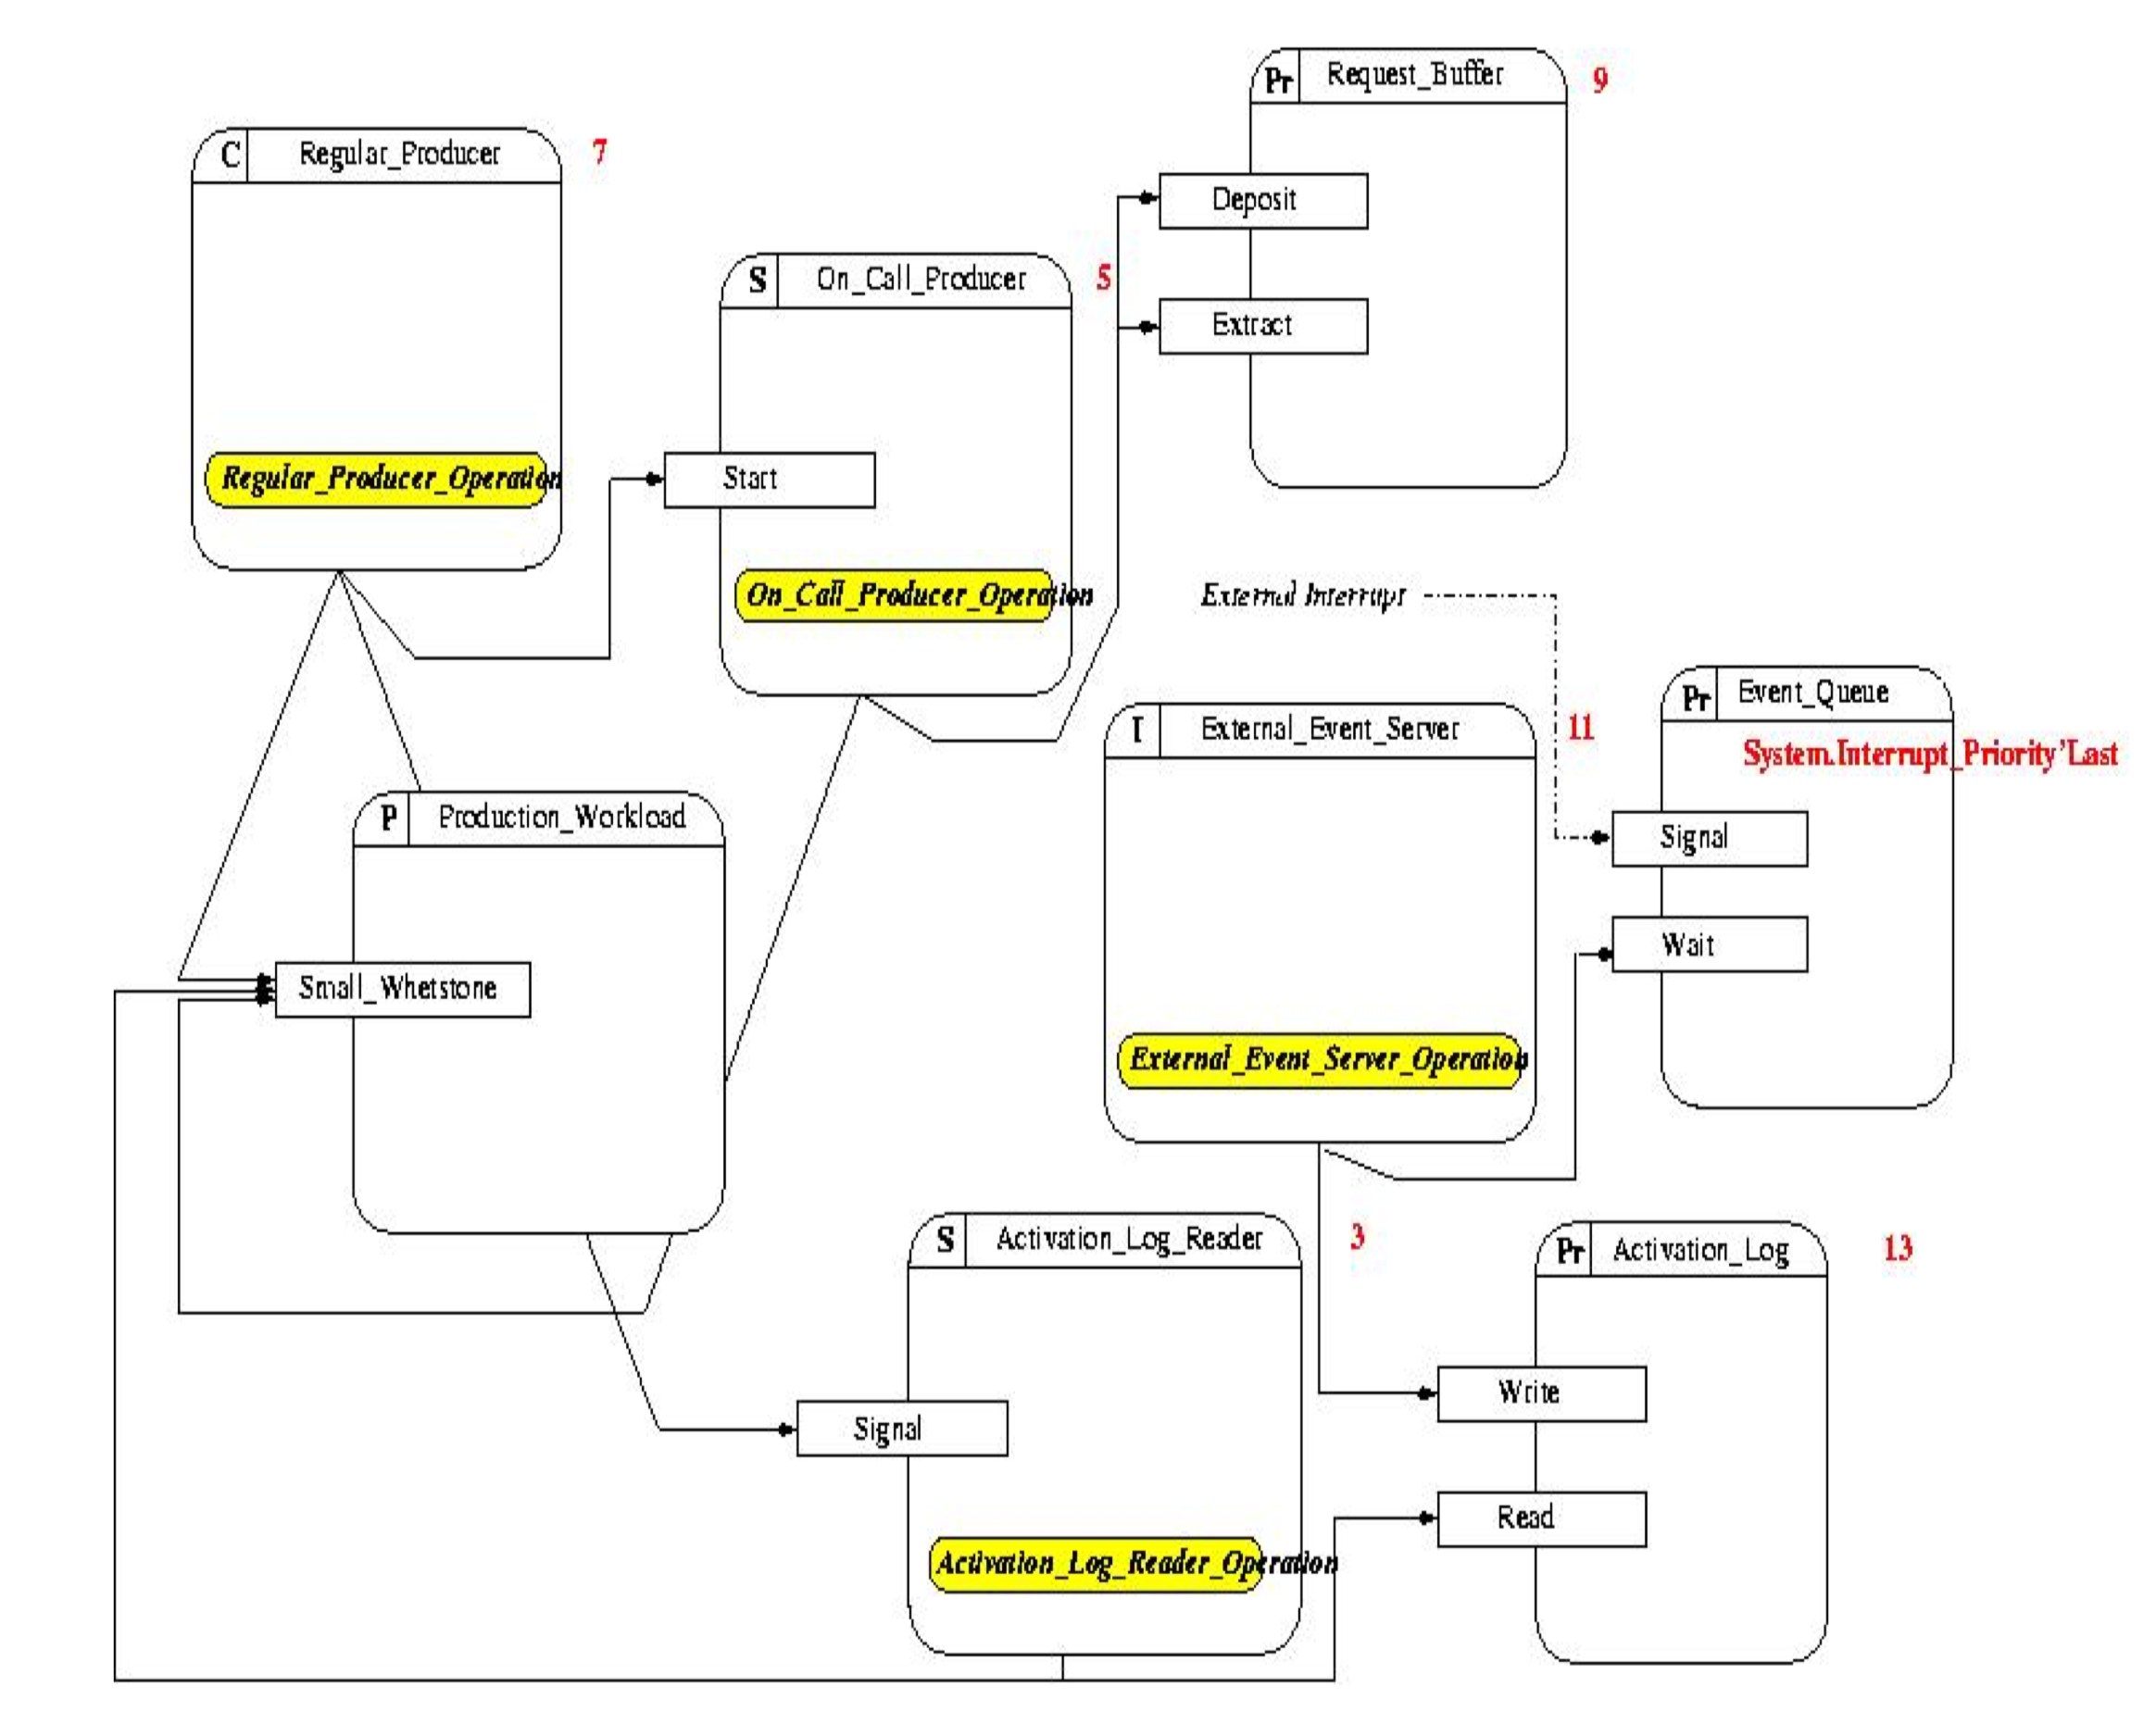
\includegraphics[width=5in]{images/ycs}
\caption{Architecture of the example application \cite{ycs}.}
\label{ycs}
\end{figure}

The example application presented in this paper is extracted from "Guide for the use of the
Ada Ravenscar Profile in
high integrity systems" \cite{ycs}. It includes a periodic process that handles orders for a variable amount of workload. Whenever the request level exceeds a certain threshold, the periodic process farms the excess load out to a supporting sporadic process. While such orders are executed, the system may receive interrupt requests from an external manual push-button. Each interrupt treatment records an entry in an activation log.

When specific conditions hold, the periodic process releases a further sporadic process to perform a check on the interrupt activation entries recorded in the intervening period. The policy of work delegation adopted by the system allows the periodic process to ensure the constant discharge of a guaranteed level of workload.

The correct implementation of this policy also requires assigning the periodic process a higher priority than those assigned to the sporadic processes, so that guaranteed work can be performed in preference to subsidiary activities.

The application is comprised by the tasks and attributes in Table \ref{tab:tasks-attributes}. Static priorities are given based on the deadline monotonic scheduling \cite{rm-dm}, which the most optimal between the fixed priority algorithms \cite{optimality-rm-dm}.

\begin{table}[!htbp]
   \centering
   \begin{tabular}{lllll}
     \toprule
     Task name & Task type & Period / Minimum inter-arrival time (ms) & Deadline (ms) & Priority  \\
     \midrule
     Regular\_Producer & Cyclic & 1000 & 500 & 7 \\
     On\_Call\_Producer & Sporadic & 3000 & 800 & 5 \\
     Activation\_Log\_Reader & Sporadic & 3000 & 1000 & 3 \\
     External\_Event\_Server & Interrupt sporadic & 5000 & 100 & 11 \\
     \bottomrule
   \end{tabular}
   \caption{Attributes of the tasks in the application \cite{ycs}}
   \label{tab:tasks-attributes}
\end{table}

Ada protected objects [RM 9.4] are used to ensure mutually exclusive access to shared resources, whereas protected entries are used only for task synchronization purposes where data exchange is involved.

In a real-time application, each protected object has a priority ceiling which represents the maximum priority of any task that calls the object. The Ada Real-Time Systems Annex supports the definition of  \texttt{Locking\_Policy} [RM D.3] and implements the resource locking protocol called Immediate Priority Ceiling Protocol (IPCP) \cite{ada-pcp}, which is similar to the Priority Ceiling Protocol (PCP).

PCP is an improvement of the Priority Inheritance Protocols (PIP) which allow a task to execute with an enhanced priority if it is blocking (or could block) a higher-priority task. In addition to PIP, PCP prevents deadlock and reduces blocking to its minimum value: every job is blocked at most once for the duration of a critical section, no matter how many jobs conflict with it \cite{pcp-blocking}.

The IPCP is similar to PCP in its use of the ceiling priority, but it has a different set of rules on how a task behaves under the ceiling locking protocol.

\begin{enumerate}
   \item A task may lock a protected object if it is not yet locked.
   \item When it enters a critical section it immediately inherits the priority ceiling of the protected object, and recovers its entry priority when it exits the section.
\end{enumerate}

This protocol effectively prevents any task from starting to execute until all the shared resources it needs are free. This means that no separate mutual exclusion mechanism, such as semaphores, is needed to lock shared resources. It is also cheap to implement at run time and incurs in less context switches. By raising priorities as soon as a resource is locked, whether a higher priority task is trying to access it or not, the protocol avoids the need to make complex scheduling decisions while tasks are already executing.

\begin{table}[!htbp]
   \centering
   \begin{tabular}{lll}
     \toprule
     Protected object names & User tasks & Ceiling priority  \\
     \midrule
     Request\_Buffer & Regular\_Producer (\texttt{Deposit}), On\_Call\_Producer (\texttt{Extract}) & 9 \\
     Event\_Queue & External interrupt (\texttt{Signal}), External\_Event\_Server (\texttt{Wait}) & System.Interrupt\_Priority'First \\
     Activation\_Log & External\_Event\_Server (\texttt{Write}), Activation\_Log\_Reader (\texttt{Read}) & 13 \\
     \bottomrule
   \end{tabular}
   \caption{Attributes of the protected objects in the application \cite{ycs}}
   \label{tab:po-attributes}
\end{table}

\section{Ada tasking model}

In the Ada Ravenscar, a periodic task has an infinite loop within which there is a self-suspension statement that ensures that the task executes regularly \cite{ada-tasks}:

\begin{lstlisting}[language=Ada]
with Ada.Real_Time; use Ada.Real_Time;
...
task Periodic_Task;
   task body Periodic_Task is
      Period : Time_Span := Milliseconds(1000);
      -- define the period of the task, 1000 ms in this example
      Next : Time;
   begin
      Next := Clock;
      -- start time
      loop
         -- undertake the work of the task
         Next := Next + Period;
         delay until Next;
      end loop;
end Periodic_Task;
\end{lstlisting}

However, we should bear in mind that \texttt{Period} is the minimum length of time between the release times of instances of the task. The subsequent jobs will be released periodically only if the loop always completes within \texttt{Period} time units. If the response time of an instance of the thread exceeds the value, the next instance is released only as soon as the current instance completes. Therefore there will be both a deadline miss of the current job and a delay in activation of the subsequent instance.

A sporadic task requires instead a protected object to control its release:

\begin{lstlisting}[language=Ada]
task Sporadic_Task;
protected Sporadic_Controller is
   entry Wait_Next_Invocation;
   procedure Release_Sporadic;
private
   Barrier : Boolean := False;
end Sporadic_Controller;

task body Sporadic_Task is
begin
   loop
      Sporadic_Controller.Wait_Next_Invocation;
      -- undertake the work of the task
   end loop;
end Sporadic_Task;

protected body Sporadic_Controller is
   entry Wait_Next_Invocation when Barrier is
   begin
      Barrier := False;
   end;

   procedure Release_Sporadic is
   begin
      Barrier := True;
   end;
end Sporadic_Controller;
\end{lstlisting}

The task body for an event-triggered task that conforms to the Ravenscar Profile typically has, as its last statement, an outermost infinite loop whose first statement is either a call to a protected entry or a call to a Suspension Object \cite{ycs}. The Suspension Object is used when no other effect is required in the signalling operation; for example, no data is to be transferred from signaller to waiter. In contrast, the protected entry is used for more elaborate event signalling, when additional operations must accompany the resumption of the event-triggered task.

\section{System model and notation}\label{model-notation}

The described application is a set of tasks executing in the same processor, grouped into entities called transactions \cite{tindell-offsets}. Each transaction $\Gamma_i$ is activated by a periodic sequence of external events with period $T_i$ , and contains a set of tasks. Each task is released when a relative time offset elapses after the arrival of the external event. Each activation of a task releases the execution of one instance of that task, called a \textit{job}.

\begin{figure}[!htbp]
\centering
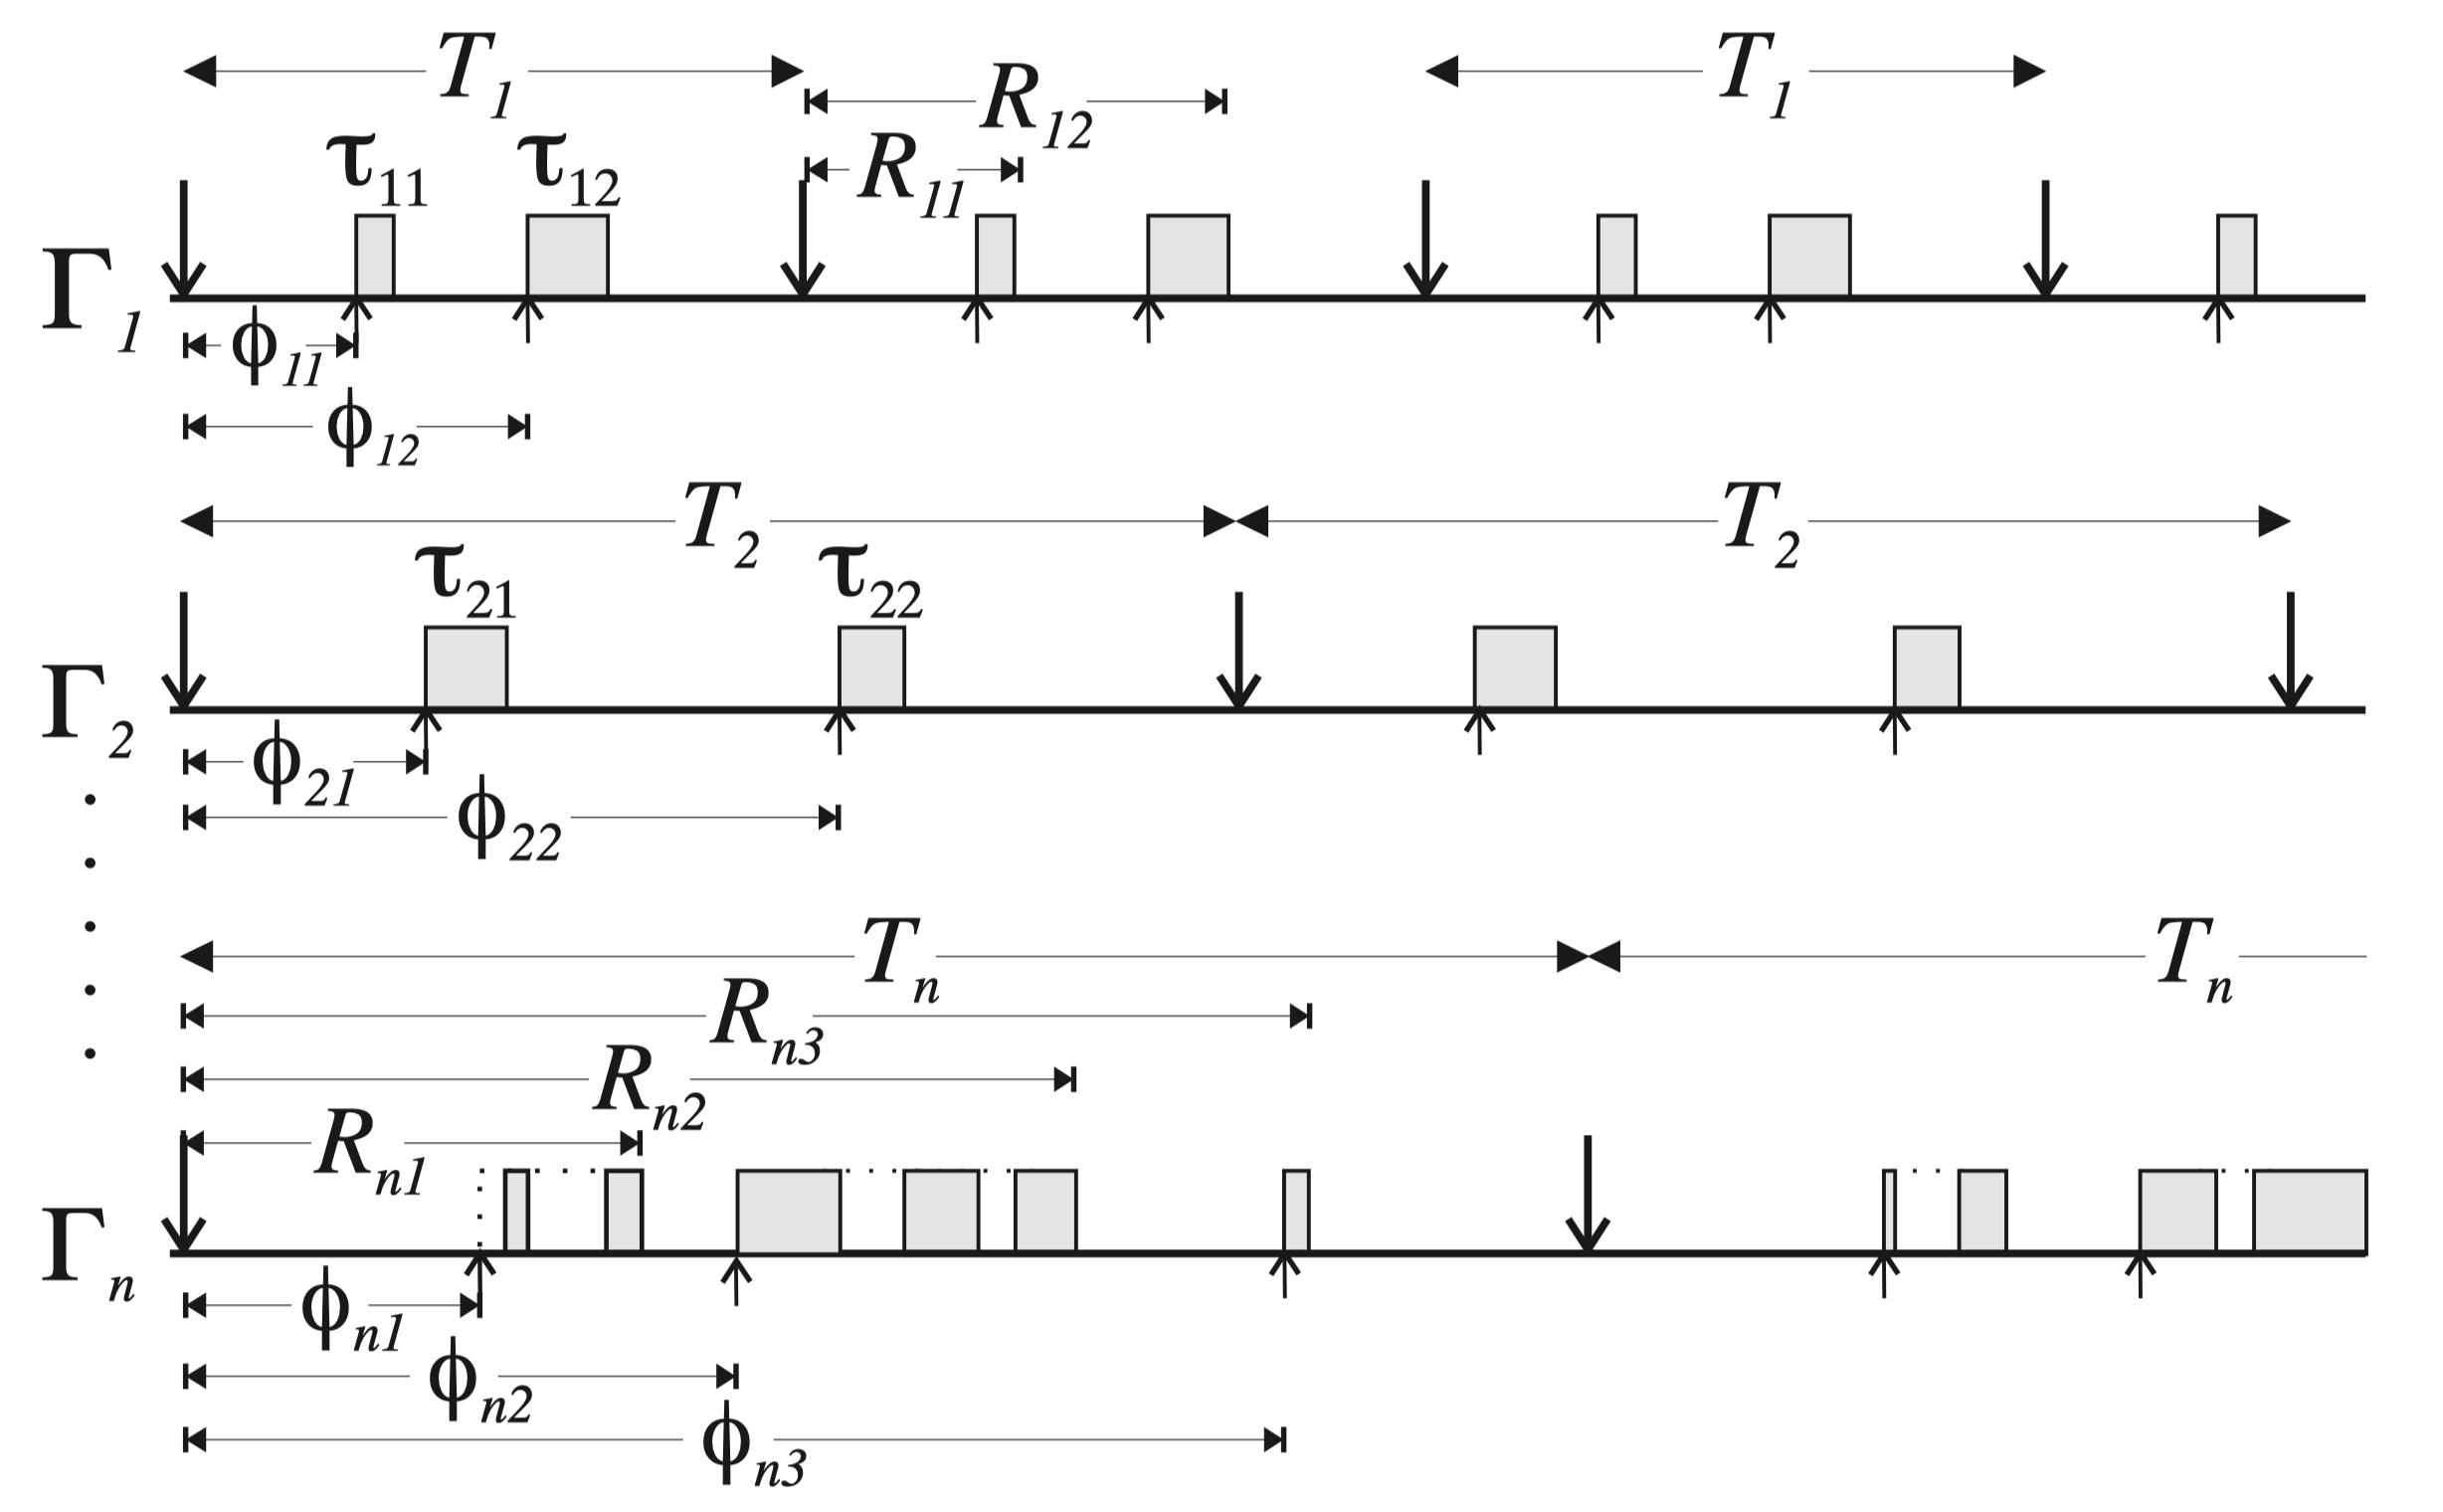
\includegraphics[width=5in]{images/transactions}
\caption{Timeline of a system composed of transactions with offsets \cite{pessimistic-rma}}
\label{transactions}
\end{figure}

Figure \ref{transactions} shows an example of such system: the horizontal axis represents time; down-pointing arrows represent the arrival of the external events associated to each transaction, while up-pointing arrows represent the activation times of each task; and shaded boxes represent task execution \cite{pessimistic-rma}. Each task has its own unique priority and in this example the task set is scheduled using a preemptive FPS.

Each task will be identified with two subscripts: the first one identifies the transaction to which it belongs, and the second one the position that the task occupies within the tasks of its transaction, when they are ordered by increasing offsets. In this way, $\tau_{ij}$ will be the j-th task of transaction $\Gamma_i$, with an offset of $\Phi_{ij}$ and a worst-case execution time of $C_{ij}$. In addition, we will allow each task to have jitter, that is to have its activation time delayed by an arbitrary amount of time between 0 and the maximum jitter for that task, which we will call $J_{ij}$. This means that the activation time of task $\tau_{ij}$ may occur at any time between $t_0 + \Phi_{ij}$ and $t_0 + \Phi_{ij} + J_{ij}$, where $t_0$ is the instant at which the external event arrived.

The reason for this is that tasks must execute in order, i.e. On\_Call\_Producer can start executing only after the preceding task in the transaction, Regular\_Producer, has completed. The precedence constraints are modeled by assigning each task an initial offset and a maximum jitter \cite{tindell-offsets}. The initial offset $\Phi_{ij}$ of a periodic task is the instant of the first activation of the task. However, a task belonging to a transaction may start only after it has been activated and the preceding task in the transaction has completed execution. Hence maximum jitter is the maximum time interval it can occur from the task activation until the completion time of the preceding task in the transaction.

In addition to maximum jitter, tasks offsets are allowed to vary dynamically, from one activation to the next, within a minimum and a maximum value: $\Phi_{ij} \in [\Phi_{ij\ min}, \Phi_{ij\ max}]$. Dynamic offsets are useful in systems in which tasks suspend themselves, like in the case of protected object entries. The task On\_Call\_Producer $\tau_{i2}$ calls the protected entry \texttt{Extract} and suspends itself until the task Regular\_Producer $\tau_{i1}$ replenishes the \texttt{Request\_Buffer}. The activation time of On\_Call\_Producer depends on the completion time of the Regular\_Producer and thus the offset for task $\tau_{i2}$ is variable in the interval $\Phi_{i2} \in [R_{i1\ min}, R_{i1\ max}]$, where $R_{i1\ min}$ and $R_{i1\ max}$ are respectively the best-case and worst-case response times of task Regular\_Producer.

For each task $\tau_{ij}$ we define its response time as the difference between its completion time and the instant at which the associated external event arrived. The worst-case response time will be called $R_{ij}$. Each task has also an associated global deadline, $D_{ij}$, which is again relative to the arrival of the external event.

If tasks synchronize using shared resources in a mutually exclusive way, they will be using the aforementioned Immediate Priority Ceiling Protocol. The effects of lower priority tasks on a task under analysis $\tau_{ab}$ are bounded by an amount called the blocking term $B_{ab}$, calculated as the maximum of all the critical sections of lower priority tasks that have a priority ceiling higher than or equal to the priority of $\tau_{ab}$.

\subsection{Offset-based analysis}

Rate monotonic analysis (RMA) \cite{rm-dm} allows an exact calculation of the worst-case response time of tasks in single-processor real time systems, including the effects of task synchronization, the presence of aperiodic tasks, the effects of deadlines before, at or after the periods of the tasks, tasks with varying priorities, overhead analysis, etc. However, classic RMA \cite{practitioner-common-data} cannot provide exact solutions in systems in which tasks suspend themselves. Classic techniques for these systems are based on the assumption that all tasks are independent, and thus they lead to pessimistic results \cite{pessimistic-rma}.

For building the worst-case scenario for a task $\tau_{ab}$ under analysis, the analysis must consider the critical instant that leads to the worst-case busy period. A task $\tau_{ab}$ busy period is an interval of time during which the CPU is busy processing task $\tau_{ab}$ or higher priority tasks. For tasks with offsets, it must take into account that the critical instant may not include the simultaneous activation of all higher priority tasks, as it was the case when all tasks were independent. The existence of offsets makes it impossible for some sets of tasks to simultaneously become active.

Works on such problem has been the base of offset-based analysis, first proposed by Tindell and Clark \cite{tindell-offsets} and later improved by Palencia and Gonzàlez \cite{pessimistic-rma} who called it Worst-Case Analysis of Dynamic Offsets. In such analysis, the best and worst-case response times of each task are used to set the offset and the jitter of the successive task in the same transaction.

\section{Execution times}

To use the described model, upper bounds on the execution times are needed. Unfortunately precise Worst-Case Execution Time (WCET) is hard to find due to pipelines, caches and other performance enhancing techniques used on contemporary computer architectures \cite{wcet-problem}. This effects are reduced in the case of a more predictable bare-board environment, which can nevertheless suffers a small amount of indeterminism. Therefore pessimistic scheduling is needed in order to provide an offline guarantee that all hard deadlines will be met, but leads to poor processor utilization.

\begin{figure}[!htbp]
\centering
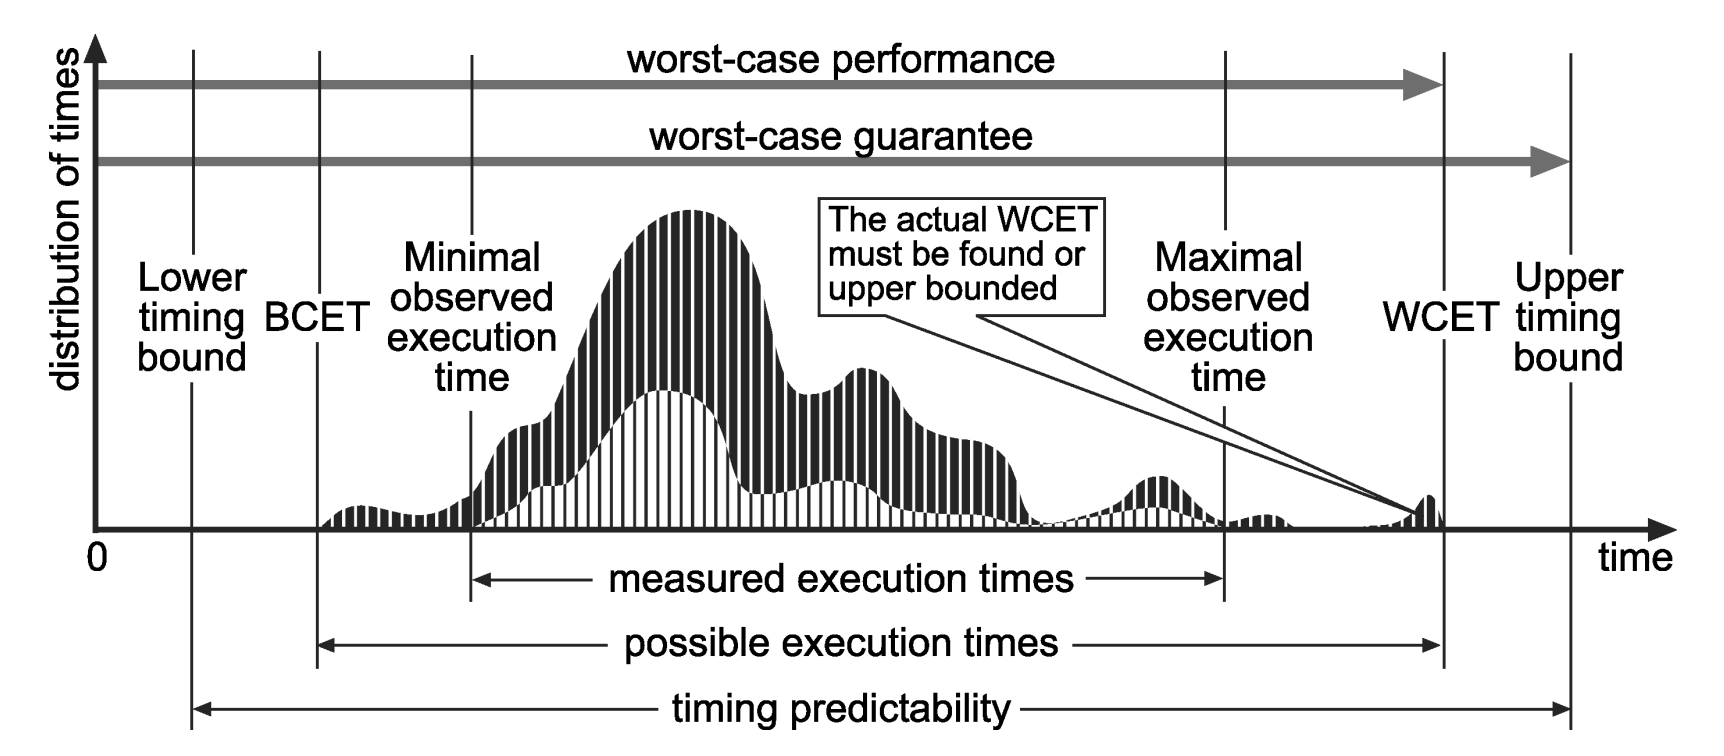
\includegraphics[width=5in]{images/wcet}
\caption{The lower curve represents a subset of measured executions. The darker curve, an envelope of the former, represents the times of all executions. \cite{wcet-problem}.}
\label{wcet-curve}
\end{figure}

Figure \ref{wcet-curve} shows the set of all execution times as the upper curve. Its minimum and maximum are the best- and worst-case execution times, respectively, abbreviated BCET and WCET. In most cases, the space is too large to exhaustively explore all possible executions and thereby determine the exact worst- and best-case execution times.

The common method to estimate execution time bounds is to measure the end-to-end execution time of the task for a subset of the possible executions. This determines the minimal observed and maximal observed execution times. These will, in general, overestimate the BCET and underestimate the WCET.

Nevertheless, we have adopted the same approach, aware of the mentioned perils. In most cases, we had deterministic execution times with always the same exact number of CPU cycles or with a difference less than 1$\mu$s, except for the Whetstone operations which showed more significant variation. However, we always had very low standard errors minor than 1\%. The example application is quite simple, comprised of few tasks with predictable executions and the only interrupts are the periodic ticker and the external push button.

Execution times are measured using two custom packages: \texttt{System\_Overhead} and \texttt{Task\_Metrics}. The former is able to provide the exact number of elapsed CPU ticks, which is then converted as seconds by dividing it with the clock frequency. It's used to measure runtime overhead, whereas the latter provides task execution time if self-suspension can happen, which would make usage of the clock ticks unsuitable.

\begin{lstlisting}[language=Ada]
-- system-overhead.ads
with System.BB.Time; use System.BB.Time;
with System.Semihosting;

package System_Overhead is
   pragma Preelaborate;

   procedure Start_Tracking;

   --  Avoid counting sub-program execution time
   procedure Start_Sub_Program;
   procedure End_Sub_Program;

   procedure End_Tracking (Item : String := "");

   procedure Log_Time;
   --  Just log the current clock time
end System_Overhead;

with System.BB.Time; use System.BB.Time;
with System.Semihosting;
\end{lstlisting}

\begin{lstlisting}[language=Ada]
-- system-overhead.adb
package body System_Overhead is
   Initial_Value : Time := 0;
   Start_Sub_Value : Time := 0;
   End_Sub_Value : Time := 0;

   procedure Start_Tracking is
   begin
      Initial_Value := Clock;
      Start_Sub_Value := 0;
      End_Sub_Value := 0;
   end Start_Tracking;

   procedure Start_Sub_Program is
   begin
      Start_Sub_Value := Clock;
   end Start_Sub_Program;

   procedure End_Sub_Program is
   begin
      End_Sub_Value := Clock;
   end End_Sub_Program;

   procedure End_Tracking (Item : String := "") is
      Now : constant Time := Clock;
      Sub_Program : Time;
      Elapsed : Time;
   begin
      -- Sometime End_Tracking may be called before Start_Tracking
      if Initial_Value = 0 then
         return;
      end if;

      Sub_Program := End_Sub_Value - Start_Sub_Value;
      Elapsed := Now - Initial_Value - Sub_Program;

      Put_Line (Item & Time'Image (Elapsed));
   end End_Tracking;

   procedure Log_Time is
   begin
      Put_Line (Time'Image (Clock));
   end Log_Time;

   procedure Put_Line (Item : String) is
   begin
      System.Semihosting.Put (Item & ASCII.CR & ASCII.LF);
   end Put_Line;
end System_Overhead;
\end{lstlisting}

The \texttt{System\_Overhead} package uses the board-specific \texttt{System.BB.Time} package, which provides the \texttt{Clock} function to read the real-time monotonic clock. It's the same primitive used under-the-hood by \texttt{Ada.Real\_Time} [RM D.8] to provide physical time as observed in the external environment.

The package \texttt{Task\_Metrics} has the same interface as \texttt{System\_Overhead}, but it replaces \texttt{System.BB.Time} with \texttt{Ada.Execution\_Time} [RM D.14] to measure the elapsed execution time of a task. The \texttt{ravenscar-full-stm32f429disco} runtime supports the Ada 2012 implementation to separately account for the execution time of interrupt handlers \cite{etc}.

The functionality of the real-time clock (RTC) and execution time clocks (ETCs) are quite similar: both clocks support high accuracy measurement of the monotonic passing of time since an epoch, and both support calling a protected handler when a given timeout time is reached. The main difference is that the RTC is always active, while an ETC is active only when its corresponding task or interrupt is executed.

\subsection{Semi-hosting}

It is worth mentioning the usage of semi-hosting \cite{semihosting}, which allows print messages to be transferred from the board to the host computer using the debug connection. Using semi-hosting for printing is usually much slower than UART because the semi-hosting mechanism needs to halt the processor, but on the other hand the system tick timer \texttt{Sys\_Tick} counter is stopped during the transmission, thus avoiding affecting the schedule of the tasks. The example application has no timing requirements relative to external interrupts, with the exception of the manual push-button.

Both \texttt{System\_Overhead} and \texttt{Task\_Metrics} use semi-hosting to send execution time data to the host computer. Besides, it is leveraged also in the \texttt{ravenscar-full-stm32f429disco} runtime implementation of the \texttt{Ada.Text\_IO} package, whose method \texttt{Put\_Line} is called by the tasks.

The runtime defines a semi-hosting buffer size of 128 characters before flushing a string, therefore we have padded all the print messages with white space to reach the fixed size of 50 characters. By doing so we have fixed execution time due to buffer insertion, simplifying MAST modeling of the \texttt{Put\_Line} operation.

\section{Deadline miss detection}

In later analysis, we will want to achieve the maximum schedulable utilization by analyzing a MAST model with low utilization and then increasing tasks utilization until the system no longer meets its deadlines. However, for design attributes to turn into system properties, we must enforce them at runtime. In particular, we have to check that the jobs of the tasks always complete before their respective deadline, to ensure consistency between the MAST analysis and the execution \cite{timing-properties}.

Fortunately, Ada 2005 introduced a lower level facility that maps a handler to a specific time without the need to use a separate task. The handler is associated with a timing event. When the event time is due, and detected by the runtime, the handler code is executed.

The most effective way for an implementation to support timing events is to execute the handlers directly from the interrupt handler of the clock \cite{timing-events}, and this is indeed what happens in \texttt{ravenscar-full-stm32f429disco}.

\begin{lstlisting}[language=Ada]
-- deadline_miss.ads
with System;
with Ada.Real_Time; use Ada.Real_Time;
with Ada.Real_Time.Timing_Events; use Ada.Real_Time.Timing_Events;

package Deadline_Miss is
   type Task_Name is (RP, OCP, ALR);
   type Deadline_Events_Array is array (Task_Name) of Timing_Event;

   protected Handler
     with Priority =>
       System.Interrupt_Priority'Last
   is
      procedure Notify_Deadline_Miss (Event : in out Timing_Event);
   end Handler;

   procedure Set_Deadline_Handler (Name : Task_Name; In_Time : in Time);
   procedure Cancel_Deadline_Handler (Name : Task_Name);
end Deadline_Miss;
\end{lstlisting}

\begin{lstlisting}[language=Ada]
-- deadline_miss.adb
with Ada.Real_Time; use Ada.Real_Time;

package body Deadline_Miss is
   Deadline_Events : Deadline_Events_Array;

   protected body Handler is
      procedure Notify_Deadline_Miss (Event : in out Timing_Event) is
      begin
         raise Program_Error with "Detected deadline miss";
      end Notify_Deadline_Miss;
   end Handler;

   procedure Set_Deadline_Handler (Name : Task_Name; In_Time : in Time) is
   begin
      Set_Handler (Deadline_Events (Name),
         In_Time, Handler.Notify_Deadline_Miss'Access);
   end Set_Deadline_Handler;

   procedure Cancel_Deadline_Handler (Name : Task_Name) is
      Cancelled : Boolean;
      pragma Unreferenced (Cancelled);
   begin
      Cancel_Handler (Deadline_Events (Name), Cancelled);
   end Cancel_Deadline_Handler;
end Deadline_Miss;
\end{lstlisting}

The implementation is based on the example shown in \cite{overrundetection} to detect deadline misses. The measured execution times include overrun detection overhead for Regular Producer, On Call Producer and Activation Log Reader.

\section{MAST}

MAST \cite{mast} is a Modeling and Analysis Suite for Real-Time Applications and its main goal is to provide an open source set of tools that enables engineers developing real-time applications to check the timing behavior of their application, including schedulability analysis with hard timing requirements.

It is designed to handle both fixed priority and dynamic priority scheduled systems, although offset-based analysis for Earliest Deadline First scheduling is still missing as of the time of writing. However, within fixed priorities, different scheduling strategies are allowed, including preemptive and non preemptive scheduling, interrupt service routines, sporadic server scheduling, and periodic polling servers.

The MAST model is designed to handle both single-processor as well as multiprocessor or distributed systems. In both cases, emphasis is placed on describing event-driven systems in which each task may conditionally generate multiple events at its completion. A task may be activated by a conditional combination of one or more events. The external events arriving at the system can be of different kinds: periodic, unbounded aperiodic, sporadic, bursty, or singular (arriving only once).

The system model facilitates the independent description of overhead parameters such as processor overheads (including the overheads of the timing services). This frees us from the need to include all these overheads in the actual application model, thus simplifying it and eliminating a lot of redundancy.

MAST provides also a graphical editor to generate the system using the MAST ASCII description, but it's still immature to be reliable and the presence of several graphical bugs causes an annoying experience. A graphical display of results is also available.

\subsection{The MAST Model}

We now proceed to describe the MAST model of the example application. In this phase, it will represent a FPS set of independent tasks, further sections will provide the needed changes to match a chain of dependant tasks or to support EDF scheduling. For a full reference to the MAST syntax, visit "Description of the MAST Model" \cite{mast-description}.

\subsubsection{Processing Resources}\label{processing-resources}

Processing Resources represent resources that are capable of executing abstract activities, including conventional CPU processors. Among its attributes we have the range of priorities valid for normal operations on that processing resource, and the speed factor. We have left the default value as speed factor, meaning that execution times will be expressed as seconds.

Normally when dealing with hard real-time analysis, we would also define only the Worst-Case Execution Time (WCET) of the operations but, since we have dynamic offsets depending on them, we include both best and worst execution times because we don't know for sure that always having the WCET corresponds to worst system performance. We may for instance have anomalies as in the case of multiple processors \cite{anomalies-multiprocessor}.

\begin{lstlisting}
Processing_Resource (
   Type                   => Regular_Processor,
   Name                   => cpu,
   Max_Interrupt_Priority => 255,
   Min_Interrupt_Priority => 241,
   Worst_ISR_Switch       => 2.578E-06,
   System_Timer           =>
      ( Type           => Ticker,
        Worst_Overhead => 3.844E-06,
        Period         => 0.001000),
   Speed_Factor           => 1.00);
\end{lstlisting}

The board is built with only one CPU, whereas the interrupt ranges are taken from the \texttt{System} package in the \texttt{ravenscar-full-stm32f429disco} runtime. Task priorities span from 1 to 240, while interrupt priorities go from 241 to 255. Thus it's possible to have at max 240 distinct task priorities, if more priorities are needed one can use the technique described in \cite{limited-priorities}.

The Interrupt Service Routine (ISR) overhead is measured as the time taken to run the \texttt{Interrupt\_Handler} in \texttt{System.BB.Board\_Support} package, without counting the execution time of the application interrupt handler. In Ada, the code in the handler itself executes at the hardware interrupt level, whereas the major part of the processing of the response to the interrupt is moved into an event response task, which executes at a software priority level with interrupts fully enabled.

The first procedure executes for a very short time-typically executing only the instructions that are strictly necessary to service the interrupt and reset the associated piece of hardware. The second one is implemented as a task that is activated from the interrupt handler and its priority is assigned as defined in Table \ref{tab:tasks-attributes}.

Both parts are not accounted into the ISR overhead. However, the overhead takes into account the management of the aforementioned Execution Time Clocks (ETC) \cite{etc}.

The system timer used by the board is Tick Scheduling \cite{tick-scheduling}, which represents a system that has a periodic clock interrupt that arrives at the system. When this interrupt arrives, all timed events whose expiration time has already passed, are activated.

Tick scheduling introduces two additional factors that must be accounted for in schedulability analysis. First, the fact that a job is ready may not be noticed and acted upon by the scheduler until the next clock interrupt. This introduces additional jitter that may delay the completion of the job.

Second, a self-suspended task is held in a queue which we will call the delay queue. When the scheduler executes, it scans the delay queue and moves the jobs that have been released since the last clock interrupt to the ready job queue and places them there in order of their priorities. Once in the ready queue, the jobs execute in priority order without intervention by the scheduler. The time the scheduler takes to scan and move the jobs introduces additional scheduling overhead. Similar overhead must be accounted for any timing events that need to be triggered.

The scheduling overhead is accounted in the analysis using the technique described in \cite{effects-runtime}. MAST can model the scheduler as a periodic task $\tau_0$ whose period is $p_0$. This task has the highest priority among all tasks in the system. Its execution time $C_0$ is the amount of time the scheduler takes to service the clock interrupt. This time is spent even when there is no job in the pending job queue.

In the \texttt{ravenscar-full-stm32f429disco} runtime, the period $p_0$ of the tick is 1ms, defined in the \texttt{System.BB.Board\_Support} package, and the worst overhead is measured as the time taken to execute \texttt{Timer\_Interrupt\_Handler}, the trap handler defined in the same package for the \texttt{Sys\_Tick} trap.

\subsubsection{Schedulers}

Schedulers represent the runtime procedures that implement the appropriate scheduling strategies to manage the amount of CPU processing capacity. They can have a hierarchical structure to model hierarchical scheduling \cite{hierarchical-scheduling}, but the example application has only one primary scheduler with fixed priority policy.

\begin{figure}[!htbp]
\centering
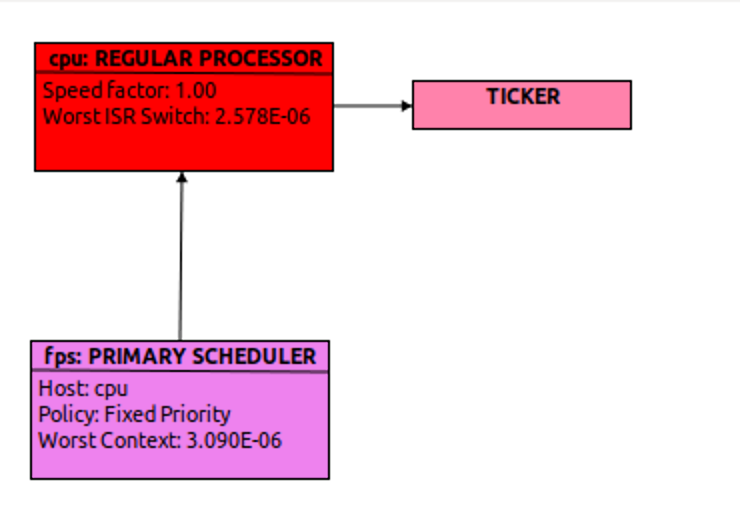
\includegraphics[width=3in]{images/primary-scheduler}
\caption{Fixed Priority Scheduler which manages the CPU}
\label{primary-scheduler}
\end{figure}

\begin{lstlisting}
Scheduler (
   Type            => Primary_Scheduler,
   Name            => fps,
   Host            => cpu,
   Policy          =>
      ( Type                 => Fixed_Priority,
        Worst_Context_Switch => 3.090E-06,
        Max_Priority         => 240,
        Min_Priority         => 1));
\end{lstlisting}

The context switch overhead is measured as time to set the context switch interrupt \texttt{Pend\_SV} as pending and the execution time of \texttt{Pend\_SV\_Handler} in the \texttt{System.BB.CPU\_Primitives.Context\_Switch\_Trigger} package, which saves the registers of active context and restores the ones of the new context. One some platforms, like in the case of the STM32F429I-Discovery board equipped with an Arm Cortex-M4 core, the context switch requires the triggering of a trap \cite{pendsv}. Then context switching is usually carried out in the \texttt{Pend\_SV} trap handler.

\subsubsection{Scheduling Servers}

Scheduling Servers represent schedulable entities in a processing resource, in particular if the resource is a processor, the scheduling server is a task or thread of control. As a matter of fact, each of them has a priority and a type, which for our application may be \texttt{Fixed\_Regular\_Policy} or \texttt{Interrupt\_FP\_Policy}. The former represents a regular preemptive fixed priority, whereas the latter models an interrupt service routine. In reality, we have not used a \texttt{Interrupt\_FP\_Policy} as the interrupt overhead is negligible.

\begin{figure}[!htbp]
\centering
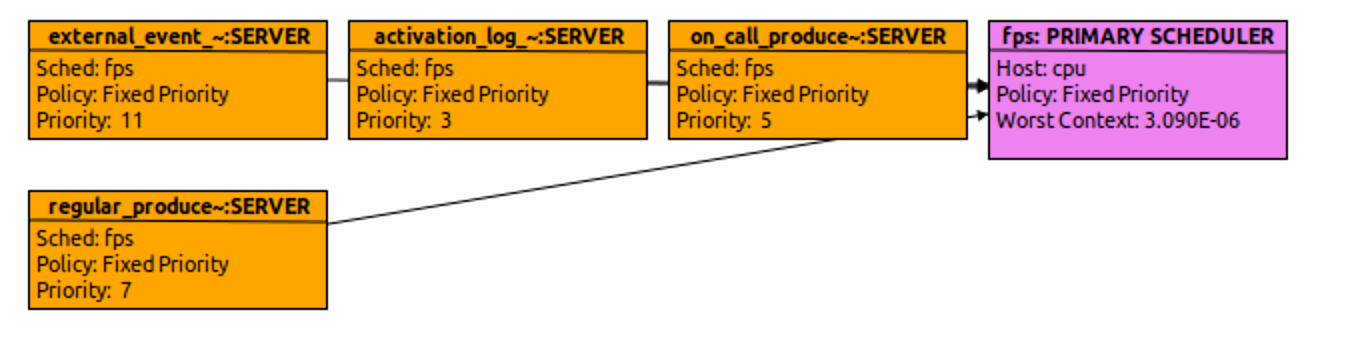
\includegraphics[width=5in]{images/scheduling-servers}
\caption{Scheduling Servers representing the application tasks}
\label{scheduling-servers}
\end{figure}

\begin{lstlisting}
Scheduling_Server (
   Type                       => Regular,
   Name                       => regular_producer,
   Server_Sched_Parameters    =>
      ( Type         => Fixed_Priority_Policy,
        The_Priority => 7,
        Preassigned  => YES),
   Scheduler                  => fps);

Scheduling_Server (
   Type                       => Regular,
   Name                       => on_call_producer,
   Server_Sched_Parameters    =>
      ( Type         => Fixed_Priority_Policy,
        The_Priority => 5,
        Preassigned  => YES),
   Scheduler                  => fps);

Scheduling_Server (
   Type                       => Regular,
   Name                       => activation_log_reader,
   Server_Sched_Parameters    =>
      ( Type         => Fixed_Priority_Policy,
        The_Priority => 3,
        Preassigned  => YES),
   Scheduler                  => fps);

Scheduling_Server (
   Type                       => Regular,
   Name                       => external_event_server,
   Server_Sched_Parameters    =>
      ( Type         => Fixed_Priority_Policy,
        The_Priority => 11,
        Preassigned  => YES),
   Scheduler                  => fps);
\end{lstlisting}

\subsubsection{Shared Resources}

Shared Resources represent resources that are shared among different tasks, and that must be used in a mutually exclusive way. Therefore, protected objects are modeled as Shared Resourses that use the Immediate Priority Ceiling Protocol described above.

\begin{figure}[!htbp]
\centering
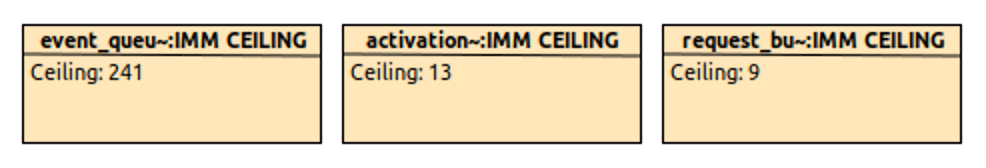
\includegraphics[width=4in]{images/shared-resources}
\caption{Shared Resources of the application}
\label{shared-resources}
\end{figure}

\begin{lstlisting}
Shared_Resource (
   Type        => Immediate_Ceiling_Resource,
   Name        => request_buffer,
   Ceiling     => 9,
   Preassigned => YES);

Shared_Resource (
   Type        => Immediate_Ceiling_Resource,
   Name        => activation_log,
   Ceiling     => 13,
   Preassigned => YES);

Shared_Resource (
   Type        => Immediate_Ceiling_Resource,
   Name        => event_queue,
   Ceiling     => 241,
   Preassigned => YES);
\end{lstlisting}

\subsubsection{Operations}

MAST Operations represent a piece of code to be executed by the processor. We have used the following classes of operations:

\begin{itemize}
   \item \textbf{Simple}: it represents a simple piece of code or a message. It may have the list of shared resources to lock before executing the operation, and the list of shared resources that must be unlocked after executing the operation. Simple Operations have been used to model methods of protected objects. The execution time is measured from the first line of the method to the last one, thus it doesn't include the runtime overhead associated with invoking protected methods.
   \item \textbf{Composite}: it represents an operation composed of an ordered sequence of other operations, simple or composite. The execution time attribute of this class cannot be set, because it is the sum of the execution times of the comprised operations.
   \item \textbf{Enclosing}: it represents an operation that contains other operations as part of its execution, but in this case the total execution time must be set explicitly; it is not the sum of execution times of the comprised operations, because other pieces of code may be executed in addition. For each protected method there is an Enclosing Operation which takes into account the overhead associated with calling protected methods. Sometimes corresponds to a method defined by the application, other times it's defined in the model specifically to include the runtime overhead. By doing so, we can define the caller procedures as simple Composite operations.
\end{itemize}

Examples of protected methods as Simple Operations:

\begin{lstlisting}
Operation (
   Type                       => Simple,
   Name                       => rb_deposit,
   Worst_Case_Execution_Time  => 2.000E-06,
   Shared_Resources_To_Lock   =>
      ( request_buffer),
   Shared_Resources_To_Unlock =>
      ( request_buffer));

Operation (
   Type                       => Simple,
   Name                       => rb_extract,
   Worst_Case_Execution_Time  => 2.000E-06,
   Shared_Resources_To_Lock   =>
      ( request_buffer),
   Shared_Resources_To_Unlock =>
      ( request_buffer));
\end{lstlisting}

Examples of Enclosing Operations including protected methods overhead:

\begin{lstlisting}
Operation (
   Type                     => Enclosing,
   Name                     => ocp_start,
   Worst_Case_Execution_Time=> 6.000E-06,
   Composite_Operation_List =>
      ( rb_deposit));

Operation (
   Type                     => Enclosing,
   Name                     => rb_extract_enclosing,
   Worst_Case_Execution_Time=> 7.000E-06,
   Composite_Operation_List =>
      ( rb_extract));
\end{lstlisting}

Complete example of the MAST representation of a job of the task Regular\_Producer:

\begin{lstlisting}
Operation (
   Type                       => Simple,
   Name                       => rp_small_whetstone,
   Worst_Case_Execution_Time  => 0.019363);

Operation (
   Type                       => Simple,
   Name                       => due_activation,
   Worst_Case_Execution_Time  => 1.000E-06);

Operation (
   Type                     => Enclosing,
   Name                     => ocp_start,
   Worst_Case_Execution_Time=> 6.000E-06,
   Composite_Operation_List =>
      ( rb_deposit));

Operation (
   Type                       => Simple,
   Name                       => check_due,
   Worst_Case_Execution_Time  => 1.000E-06);

Operation (
   Type                       => Simple,
   Name                       => alr_signal,
   Worst_Case_Execution_Time  => 5.000E-06);

Operation (
   Type                       => Simple,
   Name                       => put_line,
   Worst_Case_Execution_Time  => 1.400E-05);

Operation (
   Type                     => Composite,
   Name                     => rp_operation,
   Composite_Operation_List =>
      ( rp_small_whetstone,
        due_activation,
        ocp_start,
        check_due,
        alr_signal,
        put_line));

Operation (
   Type                     => Composite,
   Name                     => regular_producer,
   Composite_Operation_List =>
      ( overrun_detection,
        rp_operation,
        delay_until));
\end{lstlisting}

The Small\_Whetstone algorithm allows to control the computational workload of Regular\_Producer, On\_Call\_Producer and Activation\_Log\_Reader. By changing the workload parameters of \texttt{Small\_Whetstone} in the application, we will be able to test different utilisation of the system with likewise ease in updating the MAST model.

The Whetstone execution time is proportional to the workload parameter and exhibits deterministic behaviour. If we wanted to try what would happen by increasing the load of factor 10, we would just multiply the WCET in the model by 11, without the need to measure again all the Enclosing operations, since all the methods which use Whetstone are defined as Composite. However we have been careful to avoid forgetting to include any overhead in a Enclosing method and we have made sure they are not impacted by any change of the Whetstone workload.

\subsubsection{Transactions}

A Transaction represents a transaction of our model (see Section \ref{model-notation}) as a graph of event handlers and events, that represents interrelated activities executed in the system. A Transaction is defined with three different components: a list of External Events, a list of Internal Events (with their timing requirements if any), and a list of Event Handlers.

Events may be internal or external, and represent channels of event streams, through which individual event instances may be generated.

Internal Events are generated by an Event Handler. Internal Events have timing requirements, a Global Deadline relative to the arrival of a Referenced External Event. MAST allows also to use Local Deadlines, relative to the arrival of the event that activated that Event Handler. All of our deadlines are Hard Deadlines, e.g. they must be met in all cases, including the worst case.

External events model the interactions of the system with external components or devices through interrupts, signals, etc., or with hardware timing devices. They have a double role in the model: on the one hand they establish the rates or arrival patterns of activities in the system. On the other hand, they provide references for defining global timing requirements. MAST supports different arrival patterns, of which we used the following: \textit{Periodic} represents a stream of events that are generated periodically, such as from the Tick Scheduling; \textit{Sporadic} as a stream of aperiodic events that have a minimum interarrival time.

\begin{figure}[!htbp]
\centering
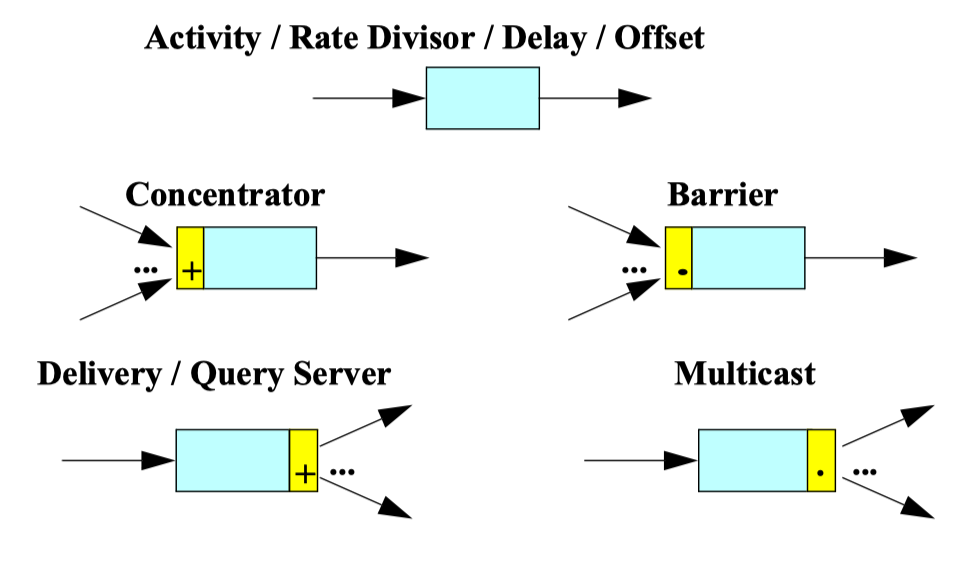
\includegraphics[width=3in]{images/event-handlers}
\caption{Event Handlers}
\label{event-handlers}
\end{figure}

Event Handlers in figure \ref{event-handlers} represent actions that are activated by the arrival of one event, and that in turn generate one or more events at their output. There are two fundamental classes of Event Handlers. The Activities represent the execution of an operation by a Scheduling Server (a task), in a processing resource (the CPU). The other kinds of Event Handlers are just a mechanism for handling events, with no runtime effects. In the model we have used the following classes:

\begin{itemize}
   \item \textit{Activity}: an instance of an operation, to be executed by a Scheduling Server;
   \item \textit{System Timed Activity}: an activity that is activated by the system timer, and thus is subject to the aforementioned jitter associated with it;
   \item \textit{Multicast}: it is an event handler that generates one event in every one of its outputs each time an input event arrives;
   \item \textit{Rate Divisor}: it is an event handler that generates one output event when a number of input events equal to the Rate Factor have arrived;
   \item \textit{Offset}: an event handler that generates its output event after a time interval has elapsed from the arrival of some (previous) external event. If the time interval has already passed when the input event arrives, the output event is generated immediately.
\end{itemize}

We now proceed to model the three transactions which model the respective independent tasks. We will start with an initial analysis of the system as stand-alone tasks, then compare its maximum utilisation with the model using dynamic offsets to represent dependant tasks.

\begin{figure}[!htbp]
\centering
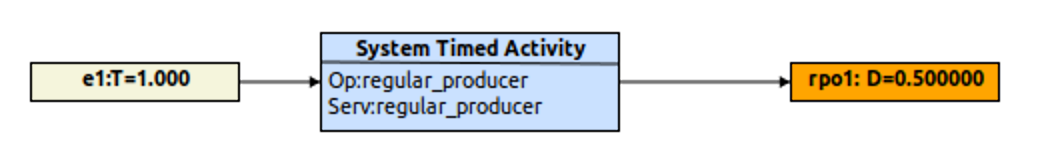
\includegraphics[width=5in]{images/transaction-rp}
\caption{Regular\_Producer transaction}
\label{transaction-rp}
\end{figure}

\begin{lstlisting}
Transaction (
   Type            => regular,
   Name            => rp_transaction,
   External_Events =>
      ( ( Type       => Periodic,
          Name       => e1,
          Period     => 1.000,
          Max_Jitter => 0.000,
          Phase      => 0.000)),
   Internal_Events =>
      ( ( Type => Regular,
          Name => rpo1,
          Timing_Requirements =>
            ( Type             => Hard_Global_Deadline,
              Deadline         => 0.500000,
              Referenced_Event => e1))),
   Event_Handlers  =>
      ( (Type               => System_Timed_Activity,
         Input_Event        => e1,
         Output_Event       => rpo1,
         Activity_Operation => regular_producer,
         Activity_Server    => regular_producer)));
\end{lstlisting}

The main event stream is modeled as a transaction activated by the periodic system timer, with period of 1s. The event is handled by the \texttt{regular\_producer} operation, representing a job of the same name. The Event Handler is of type \texttt{System\_Timed\_Activity} to take into account the jitter caused by the tick scheduling.

\begin{figure}[!htbp]
\centering
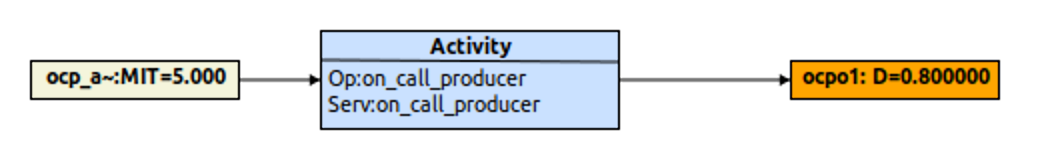
\includegraphics[width=5in]{images/transaction-ocp}
\caption{On\_Call\_Producer transaction}
\label{transaction-ocp}
\end{figure}

\begin{figure}[!htbp]
\centering
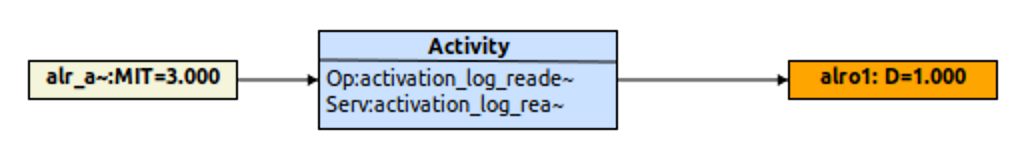
\includegraphics[width=5in]{images/transaction-alr}
\caption{Activation\_Log\_Reader transaction}
\label{transaction-alr}
\end{figure}

\begin{lstlisting}
Transaction (
   Type            => regular,
   Name            => ocp_transaction,
   External_Events =>
      ( ( Type             => Sporadic,
          Name             => ocp_activation,
          Avg_Interarrival => 5.000,
          Distribution     => UNIFORM,
          Min_Interarrival => 5.000)),
   Internal_Events =>
      ( ( Type => Regular,
          Name => ocpo1,
          Timing_Requirements =>
            ( Type             => Hard_Global_Deadline,
              Deadline         => 0.800000,
              Referenced_Event => ocp_activation))),
   Event_Handlers  =>
      ( (Type               => Activity,
         Input_Event        => ocp_activation,
         Output_Event       => ocpo1,
         Activity_Operation => on_call_producer,
         Activity_Server    => on_call_producer)));
\end{lstlisting}

The sporadic On\_Call\_Producer event stream is modeled as activated by a bounded aperiodic event, with minimum interarrival time of 5s and uniform distribution. Actually we know that the interarrival time is precisely 5s, thus the same value as average interarrival time. Similar modelling has been done for the Activation\_Log\_Reader sporadic task.

\begin{figure}[!htbp]
\centering
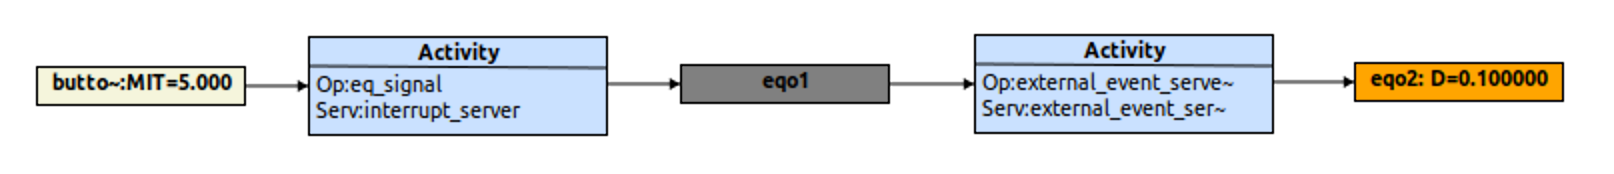
\includegraphics[width=6in]{images/transaction-eq}
\caption{External push-button transaction}
\label{transaction-eq}
\end{figure}

\begin{lstlisting}
Transaction (
   Type            => regular,
   Name            => interrupt_transaction,
   External_Events =>
      ( ( Type             => Sporadic,
          Name             => button_click,
          Avg_Interarrival => 0.000,
          Distribution     => UNIFORM,
          Min_Interarrival => 5.000)),
   Internal_Events =>
      ( ( Type => Regular,
          Name => eqo1,
          Timing_Requirements =>
            ( Type             => Hard_Global_Deadline,
              Deadline         => 0.100000,
              Referenced_Event => button_click))),
   Event_Handlers  =>
      ( (Type               => Activity,
         Input_Event        => button_click,
         Output_Event       => eqo1,
         Activity_Operation => external_event_server,
         Activity_Server    => external_event_server)));
\end{lstlisting}

The push-button interrupt event stream is modeled as triggered by a sporadic event of 5s as minimum interarrival time and it's handled by the \texttt{external\_event\_server} job at software priority. The interrupt handler at hardware interrupt priority has not been modeled since it's execution time is negligible.

\section{MAST analysis}

As of the time of writing, MAST is at version 1.5.1 and supports the analysis tools \cite{mast-analysis} in Figure \ref{mast-analysis-tools}. The techniques relevant for this paper are:

\begin{figure}[!htbp]
\centering
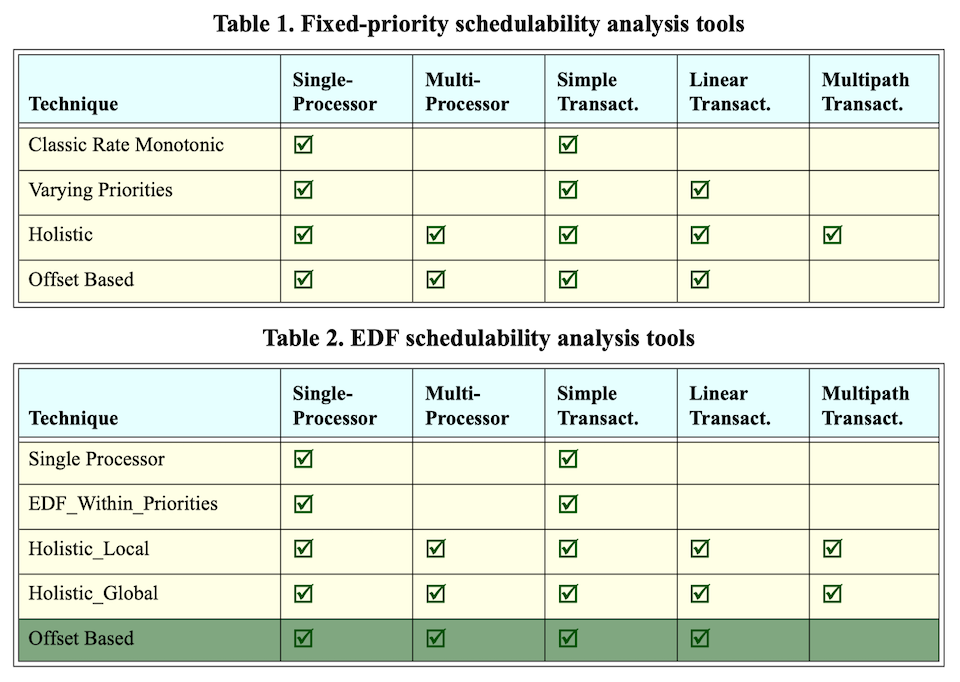
\includegraphics[width=5in]{images/mast-analysis}
\caption{MAST analysis tools \cite{mast-analysis}.}
\label{mast-analysis-tools}
\end{figure}

\begin{itemize}
   \item \textit{Classic RM Analysis}: it implements the classic exact response time analysis for single-processor fixed-priority systems and corresponds to the Technique "Calculating response time with arbitrary deadlines and blocking" in \cite{practitioner};
   \item \textit{Holistic Analysis}: this analysis extends the response time analysis to multiprocessor and distributed systems. It is not an exact analysis, because it makes the assumption that tasks of the same transaction are independent. It was first developed for fixed priority systems by Tindell and Clark \cite{holistic-analysis}. It has no use for our purposes, but it is worth mentioning to the reader because it can support both FPS and EDF monoprocessor and has less restrictions compared to \textit{Classic RM Analysis}, as explained below. In terms of our example application, both techniques provides equivalent results;
   \item \textit{EDF Monoprocessor / Single Processor}: it implements the exact response time analysis for single-processor EDF systems first developed by Spuri \cite{spuri};
   \item \textit{Offset Based Approximate Analysis}: this is a response time analysis for multiprocessor and distributed systems that improves the pessimism of the holistic analysis by taking into account that tasks of the same transaction are not independent, through the use of offsets. Offset based analysis for fixed priorities was first introduced by Tindell \cite{tindell-offsets} and then extended to distributed systems by Palencia and González \cite{pessimistic-rma};
   \item \textit{Offset Based Approximate with Precedence Relations Analysis}: this is an enhancement of the offset based approximate analysis for fixed priority systems in which the priorities of the tasks of a given transaction are used together with the precedence relations among those tasks to provide a tighter estimation of the response times;
   \item \textit{Offset Based Slanted Analysis}: this is another enhancement of the offset based approximate analysis for fixed priority systems in which the maximum interference function is defined with a tighter approximation. This method provides better results that the Offset-Based Approximate Analysis, but it is uncertain if it gets better results than the method with precedence relations.
\end{itemize}

In addition, the analysis tools are subject to different restrictions \cite{mast-restrictions}. The most significant ones are:

\begin{itemize}
   \item \textit{No\_Hard\_Local\_Deadlines}: Hard Local Deadlines cannot be used as Timing Requirements;
   \item \textit{Referenced\_Events\_Are\_External\_Only}: no internal events can be referenced by Global Deadlines;
   \item \textit{Simple\_Transactions\_Only}: checks that every transaction has only a continuous sequence of activities executed by the same server. This restriction is required by the Rate Monotonic analysis and the EDF Monoprocessor analysis;
   \item \textit{Linear\_Plus\_Transactions\_Only}: less restrictive than \textit{Simple\_Transactions\_Only}, checks that every transaction only has one external event and is not multipath, e.g. it has no Multicasts. This restriction is required by the Holistic Analysis and the different Offset based analysis tools;
   \item \textit{Restricted\_Multipath\_Transactions\_Only}: checks that every transaction has a single input event, has no branch elements (Delivery or Query Servers), and has no Rate Divisors. It also checks that the transaction follows the set of allowed constructs mentioned in \cite{mast-restrictions}. This restriction is required by the Holistic analysis.
\end{itemize}

The transaction which defines the button interrupt event stream is considered as a linear transaction, since it only has one external event, but unfortunately it is not a Simple transaction since Activities are not executed by the same server. An Interrupt Scheduling Server first handles the Interrupt Service Routine and then a regular Scheduling Server executes the application handler defined by External\_Event\_Server.

As a consequence, it's not possible to use the classic Rate Monotonic algorithm \cite{rm-dm} with our model and we are restricted to the traditional Holistic and the Offset-based tools. We believe the reason is that the Rate Monotonic assumes independent tasks, but the interrupt transaction is composed by an ISR executed by the Interrupt\_FP\_Server, followed by the interrupt handler in External Event Server, which is activated by the former and thus dependent on it for its activation.

As final note, as of the time of writing, offset-based analysis with EDF tasks fallbacks to holistic analysis \cite{mast-analysis}, which in turn does not support shared resources in EDF yet.

\section{FPS analysis}

We start the analysis with fixed priority scheduling (FPS) and a MAST model which represents the tasks as stand-alone. Later, we will try to more strictly model the formal transactions comprised of dependent tasks.

To check that the system meets the deadlines, it suffices to run it for at least the first hyperperiod amount of time. Assuming sporadic tasks as periodic with period equal to the minimum interarrival time, which is the worst case, the hyperperiod is $LCM(1, 3, 5) = 15s$. The hyperperiod of a set of tasks is least common multiple of all periods.

\subsection{Independent tasks}

We start with an Holistic analysis of the initial system.

\begin{lstlisting}
Optimum Resource Ceilings and Levels:
request_buffer =>  7
activation_log =>  11
event_queue =>  241
\end{lstlisting}

A first analysis suggests that smaller values can be used as ceilings for the protected objects Request\_Buffer and Activation\_Log. This possible improvement is expected since the two values are the highest priorities of the tasks Regular\_Producer and External\_Event\_Server respectively. We leave the ceilings intact nevertheless, since the ceiling is a required to be an upper bound of the priorities between the tasks the request the resource, not the least upper bound. Having some spare priorities between the task priorities and the ceilings might prove to be useful if we need to separate a task into two distinct tasks with proper offset to better model the application \cite{tindell-offsets}.

\begin{longtable}{llllll}
   \toprule
   Task & WCET \\
   \midrule
   regular\_producer & 0.019333 \\
   on\_call\_producer & 0.007126 \\
   activation\_log\_reader & 0.003582 \\
   \toprule
   \toprule
   Transaction & $R_{max}$ & Slack & Worst blocking time & Jitter \\
   \midrule
   rp\_transaction & 0.020434  & 2470.0\% &  2.000E-06 & 0.001101 \\
   ocp\_transaction & 0.026592 & 10776.6\% & 1.000E-06 & 0.019472 \\
   alr\_transaction & 0.030195 & 26600.8\% & 0.00 & 0.026613 \\
   interrupt\_transaction & 2.102E-05 & >=100000.0\% & 1.000E-06 & 1.102E-05 \\
   \toprule
   \toprule
   System slack & 2401.2\% \\
   Total utilisation & 2.68\% \\
   \bottomrule
\caption{Rate Monotonic analysis results for FPS}
\label{tab:rm-fps}
\end{longtable}

Table \ref{tab:rm-fps} first shows the WCET of the tasks as defined in the MAST model and which are controlled by the Whetstone workloads. Then the results of the analysis are displayed, containing the worst-case response time $R_{max}$, the slack, the blocking time and the jitter for each transaction. The MAST analysis tool provides also best-case response times $R_{min}$, but Rate Monotonic is a pessimistic analysis which assumes worst-case scenario at the critical istant, therefore only worst-case response time matters.

All transactions suffer jitter due to the system ticker interrupt running at the highest interrupt priority and the context switch overhead.

\begin{itemize}
   \item \textit{regular\_producer}: suffers additional jitter due to the system clock with granularity 1ms and the possible execution of the interrupt handler. Its blocking time is caused by the On\_Call\_Producer and the Activation\_Log\_Reader which have lower priorities but can access resources with higher ceiling priority than Regular\_Producer;
   \item \textit{ocp\_transaction}: suffers additional jitter due to interference by Regular\_Producer and the ISR. Its blocking time is caused the Activation\_Log\_Reader.;
   \item \textit{alr\_transaction}: suffers additional jitter due to interference by On\_Call\_Producer, Regular\_Producer and the ISR. It has no blocking time since it's the task with lowest priority;
   \item \textit{interrupt\_transaction}: it's the software level handler of the interrupt. It suffers no additional jitter other than the aforementioned overheads. Its blocking time is caused by the Activation\_Log\_Reader;
\end{itemize}

We shall now increase the Whetstone workload of factor 24 in the first three transactions, since 2477.0\% is the smallest slack of the three of them. The factor correponds to how much the execution time of all event responses can be increased while preserving system schedulability \cite{practitioner-growth}. We leave the Event\_Queue transaction intact because it doesn't contain any Whetstone operation. The new results are as shown in table \ref{tab:rm-fps-24}.

\begin{longtable}{llllll}
   \toprule
   Task & WCET \\
   \midrule
   regular\_producer & 0.482597 \\
   on\_call\_producer & 0.177482 \\
   activation\_log\_reader & 0.088702 \\
   \toprule
   \toprule
   Transaction & $R_{max}$ & Slack & Worst blocking time & Jitter \\
   \midrule
   rp\_transaction & 0.485486  & 2.73\% &  2.000E-06 & 0.002889 \\
   ocp\_transaction & 0.662657 & 76.95\% & 1.000E-06 & 0.485175 \\
   alr\_transaction & 0.751706 & 277.34\% & 0.00 & 0.663004 \\
   interrupt\_transaction & 2.102E-05 & >=100000.0\% & 1.000E-06 & 1.102E-05 \\
   \toprule
   \toprule
   System slack & 3.21\% \\
   Total utilisation & 57.52\% \\
   \bottomrule
   \caption{Rate Monotonic analysis results for FPS increased of factor 24}
\label{tab:rm-fps-24}
\end{longtable}

The blocking times have not changed because protected operations are same as before, but the total utilisation have increased up to 57.52\%. The 2.73\% slack value of Regular\_Producer is already very low so we can leave it as it is. We proceed instead to increase the workload of On\_Call\_Producer and Activation\_Log\_Reader from factor 24 to $43\ =\ 24\ *\ 1.77$, using the slack value 77\%.

\begin{longtable}{llllll}
   \toprule
   Task & WCET \\
   \midrule
   regular\_producer & 0.482597 \\
   on\_call\_producer & 0.312341 \\
   activation\_log\_reader & 0.156086 \\
   \toprule
   \toprule
   Transaction & $R_{max}$ & Slack & Worst blocking time & Jitter \\
   \midrule
   rp\_transaction & 0.485486  & 0.390625\% &  2.000E-06 & 0.002889 \\
   ocp\_transaction & 0.798039 & 0.390625\% & 1.000E-06 & 0.485698 \\
   alr\_transaction & 0.954730 & 28.13\% & 0.00 & 0.798644 \\
   interrupt\_transaction & 2.102E-05 & >=100000.0\% & 1.000E-06 & 1.102E-05 \\
   \toprule
   \toprule
   System slack & 0.390187\% \\
   Total utilisation & 64.26\% \\
   \bottomrule
   \caption{Rate Monotonic analysis results for FPS increased of factor 43}
\label{tab:rm-fps-24-ocp-44}
\end{longtable}
 
The system has reached utilisation 64.26\%. We now increase workload of Activation\_Log\_Reader from factor 43 to $55\ =\ 43 * 1.28$, using the slack value 28\%.

\begin{longtable}{llllll}
   \toprule
   Task & WCET \\
   \midrule
   regular\_producer & 0.482597 \\
   on\_call\_producer & 0.312341 \\
   activation\_log\_reader & 0.198645 \\
   \toprule
   \toprule
   Transaction & $R_{max}$ & Slack & Worst blocking time & Jitter \\
   \midrule
   rp\_transaction & 0.485492  & 0.0\% &  2.000E-06 & 0.002889 \\
   ocp\_transaction & 0.798039 & 0.390625\% & 1.000E-06 & 0.485698 \\
   alr\_transaction & 0.997454 & 0.390625\% & 0.00 & 0.798809 \\
   interrupt\_transaction & 2.102E-05 & >=100000.0\% & 1.000E-06 & 1.102E-05 \\
   \toprule
   \toprule
   System slack & 0.390187\% \\
   Total utilisation & 65.68\% \\
   \bottomrule
   \caption{Rate Monotonic analysis results for FPS increased of factor 55}
\label{tab:rm-fps-24-ocp-44-alr-56}
\end{longtable}

The maximum utilisation reached is about 65.68\%. The only transaction with significant slack left is \texttt{event\_queue}, but tests show that an increase of the WCET of factor 140 in the operation \textit{external\_event\_server} would improve the utilisation only up to 61.54\%, hence we can ignore it.

\subsection{Adding offsets}

So far, tasks have been assumed to be scheduled independently, there are no relationships between the release of any pair of tasks. Consequently, the worst-case task release pattern has been assumed in the critical instants \cite{critical-instants}; the resulting analysis is therefore sufficient for any task release pattern. It may, however, be advantageous to specify timing constraints on release patterns. We try to include time offsets into the computational model and, by taking account of time offsets, we try to reduce the pessimism when bounding the timing behaviour of the system.

By assuming all tasks are independent, the current analysis is subject to two pessimistic points:

\begin{enumerate}
   \item Critical instant: for tasks with offsets, we must take into account that the critical instant may not include the simultaneous activation of all higher priority tasks, as it was the case when all tasks were independent. The existence of offsets makes it impossible for some sets of tasks to simultaneously become active \cite{pessimistic-rma};
   \item Blocking time: offsets can be used to avoid the need for a dynamic concurrency control protocol for access to shared resources. Two tasks in the same transaction may not need to use locks to guard access to a shared resource if certain constraints on response times and offsets hold \cite{tindell-offsets}.
\end{enumerate}

The above pessimism can be avoided by modeling the precedence constraint: within a pair of tasks, one of them must complete execution before the other can be permitted to commence. If it can be shown that two tasks execute in exclusion then any resources shared exclusively between these tasks need not be guarded by locks, the tasks are guaranteed never to access the shared resource concurrently. Besides, the two tasks cannot be active concurrently, which means that neither task can be permitted to preempt the other causing interference in the critical instant.

\subsubsection{Critical instant}

Offsets can be used to express precedence contraints: the existence of offsets makes it impossible for some sets of tasks to simultaneously become active. This is achieved by "spreading out" the computation of tasks so that all the tasks are not released together.

In our system, the task On\_Call\_Producer (OCP) is actually not truly sporadic given that it's activated by the Regular\_Producer (RP) every 3 jobs. The two tasks are not thus independent and both the RP job which activates OCP and the latter should belong to the same transaction. Equivalent argument holds true for the RP job that awakens Activation\_Log\_Reader (ALR). The remaining instances of the RP tasks should belong to another transaction again.

Formally, for the two tasks RP and OCP that are members of the same transaction, task RP must complete before task OCP is run. We have in theory two possible priority situations: task RP is of higher priority, or task OCP is of higher priority. Fortunately, in our system RP is the one of higher priority, which means that task OCP (of lower priority) will simply not execute if task RP has been released before task OCP and has remaining computation. It can be seen that the condition for the precedence constraint to be met is \cite{tindell-offsets}:

$\Phi_{RP}\ +\ J_{RP}\ \le\ \Phi_{OCP}$

MAST Offset-based analysis tools are able to derive such condition from the following representations of the the newly described transactions.

\begin{figure}[!htbp]
\centering
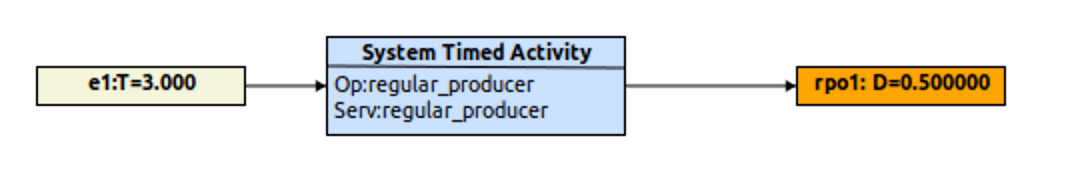
\includegraphics[width=5in]{images/transaction-rp-offset}
\caption{\texttt{regular\_producer} transaction}
\label{transaction-rp-offset}
\end{figure}

The {regular\_producer} transaction has a period of 3, representing the stand-alone RP instance.

\begin{figure}[!htbp]
\centering
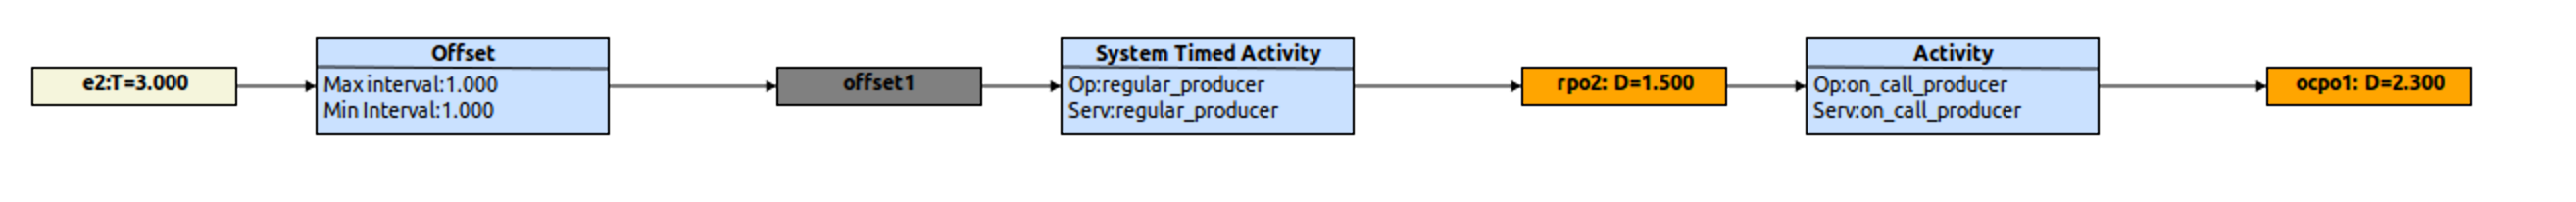
\includegraphics[width=6.5in]{images/transaction-ocp-offset}
\caption{\texttt{on\_call\_producer} transaction}
\label{transaction-ocp-offset}
\end{figure}

\begin{figure}[!htbp]
\centering
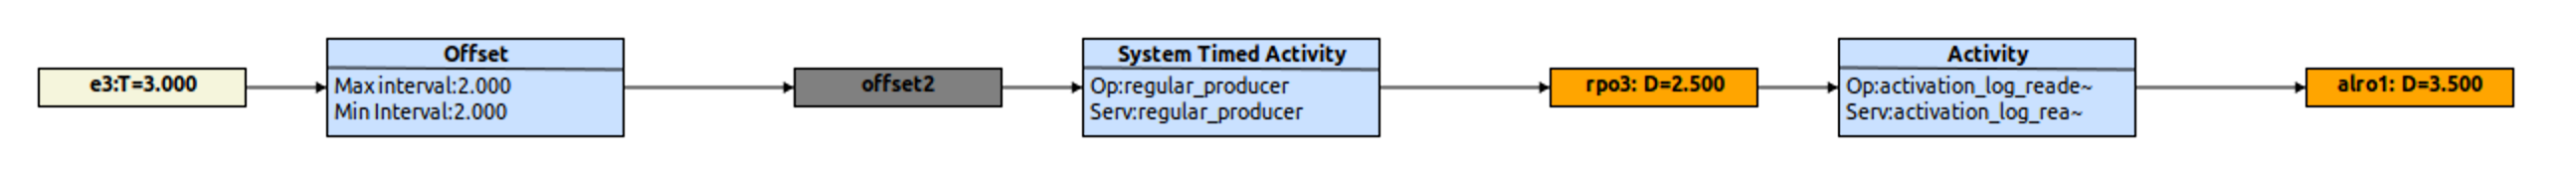
\includegraphics[width=6.5in]{images/transaction-alr-offset}
\caption{\texttt{activation\_log\_reader} transaction}
\label{transaction-alr-offset}
\end{figure}

The {on\_call\_producer} and {activation\_log\_reader} transactions have also a period of 3 and include the RP job which activates the OCP and ALR jobs respectively. Both transactions have an initial offset from the external periodic event to differentiate each RP instance from the others.

The unfolding the of three transactions reproduces the timeline in Figure \ref{timeline-offsets}, assuming the Whetstone values reached by the previous analysis. It is clear from the timeline that there is possibility for the OCP and ALR jobs to expand their execution further without provoking any deadline miss. Nevertheless, the pessimistic Rate Monotonic analysis returns zero slack because of the possible interference between stand-alone tasks.

\begin{figure}[!htbp]
\centering
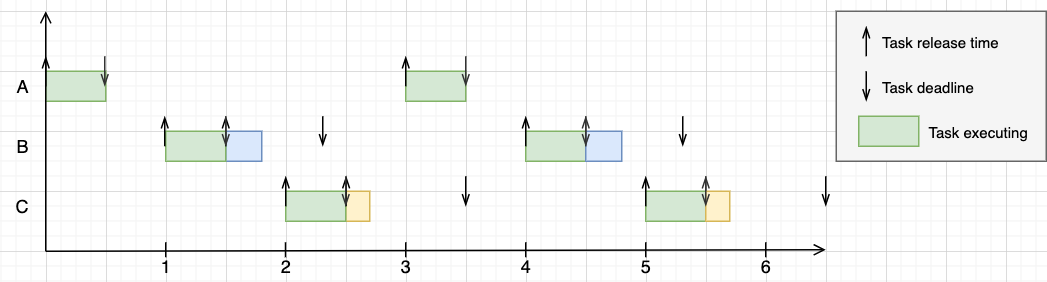
\includegraphics[width=6.5in]{images/timeline-offsets}
\caption{Unfolded timeline}
\label{timeline-offsets}
\end{figure}

As can be seen below, the Offset Based Slanted analysis provides an improvement of the best response times. Offset-based analysis tools are able to consider the offset values so that chained tasks are not released together.

\begin{longtable}{lllllll}
   \toprule
   Task & WCET \\
   \midrule
   regular\_producer & 0.482597 \\
   on\_call\_producer & 0.312341 \\
   activation\_log\_reader & 0.198645 \\
   \toprule
   \toprule
   Transaction & $R_{min}$ & $R_{max}$ & Slack & Worst blocking time & Jitter \\
   \midrule
   rp\_transaction & 0.482597 & 1.454 & -66.02\% &  2.000E-06 & 0.971820 \\
   ocp\_transaction RP & 1.483 & 2.454 & -66.02\% & 2.000E-06 & 0.971820 \\
   ocp\_transaction OCP & 1.795 & 3.737 & -66.02\% & 1.000E-06 & 1.942 \\
   alr\_transaction RP & 2.483 & 3.454 & -66.02\% & 2.000E-06 & 0.971820 \\
   alr\_transaction ALR & 2.681 & 4.936 & -66.02\% & 0.00 & 2.255 \\
   interrupt\_transaction & 1.000E-05 & 2.102E-05 & -100.0\% & 1.000E-06 & 1.102E-05 \\
   \toprule
   \toprule
   System slack & -65.55\% \\
   Total utilisation & 65.68\% \\
   \bottomrule
   \caption{Offset Based Slanted analysis results}
\label{tab:rm-fps-24-ocp-44-alr-56}
\end{longtable}

Both the $R_{min}$ and $R_{max}$ response times produced by the analysis include the initial offsets of the transaction, but the former RP $R_{min}$ values are also used as offset $\Phi_{ij}$ of the dependant tasks OCP and ALR for their respective response times. The $R_{max}$ values are instead the sum of the corresponding $R_{min}$ and jitter.

Between $R_{min}$ and $R_{max}$ response times, we consider only the best-case response time $R_{min}$. The timeline in Figure \ref{timeline-offsets} clearly shows that the three transactions have the same source of activation, a RP job, and there is no interference between tasks. Thus there cannot be any significant jitter and only the $R_{min}$ value is valuable for our considerations since it already takes into account the offsets and examines the actual case with zero interference. Besides, by not considering the worst-case response times, we ignore the slack values as well. If the best-case response time is within the deadline then it's sufficient for our considerations.

To be thorough, we provide a possible explanation of the jitters. The RP jitters are calculated as the best-case response time $R_{min}$ of the RP itself, multiplied by two as possible interference from the same task as activator of the other two transactions, whereas the difference $R_{RP\ max} - R_{RP\ min}$ is counted as possible additional jitter. I.e. the jitter suffered by a OCP instance in the transaction $B$ is $J_{B, OCP} = J_{B, RP} + R_{B, RP\ max} - R_{B, RP\ min}$.

\begin{table}[!htbp]
  \centering
  \begin{tabular}{llllll}
   \toprule
   Task & WCET \\
   \midrule
   regular\_producer & 0.482597 \\
   on\_call\_producer & 0.312341 \\
   activation\_log\_reader & 0.198645 \\
   \toprule
   \toprule
   Transaction & $R_{min}$ & $R_{max}$ & Slack & Worst blocking time & Jitter \\
   \midrule
   rp\_transaction & 0.482597 & 1.454 & -66.02\% &  2.000E-06 & 0.971820 \\
   ocp\_transaction RP & 1.483 & 2.454 & -66.02\% & 2.000E-06 & 0.971820 \\
   ocp\_transaction OCP & 1.795 & \textbf{2.768} & -66.02\% & 1.000E-06 & \textbf{0.973028} \\
   alr\_transaction RP & 2.483 & 3.454 & -66.02\% & 2.000E-06 & 0.971820 \\
   alr\_transaction ALR & 2.681 & \textbf{3.967} & -66.02\% & 0.00 & \textbf{1.286} \\
   interrupt\_transaction & 1.000E-05 & 2.102E-05 & -100.0\% & 1.000E-06 & 1.102E-05 \\
   \toprule
   \toprule
   System slack & -65.55\% \\
   Total utilisation & 65.68\% \\
  \end{tabular}
  \caption{Offset Based Approximate with Precedence Relations analysis results }
  \label{tab:off-approx-w-pr-fps}
\end{table}

Compared to Offset Based Slanted, Offset Based Approximate with Precedence Relations analysis is able to provide even tighter worst-case response times by using the precedence relation and therefore considering a dynamic offset $\Phi_{i2} \in [R_{ISR\ min}, R_{ISR\ max}]$. I.e. the OCP task is never activated before the RP completion, therefore its jitter can be approximately reduced to $J_{B, OCP} = J_{B, RP}$.

Future analysis in this section will provide only the results from the Offset Based Approximate with Precedence Relations technique, referred only as Offset-based analysis, as it has proved to be the best of the two tools even if are interested only in best-case response times.

\subsubsection{Blocking time}

We can further improve the analysis by reducing unnecessary blocking time: the precedence constraint between the RP and OCP means the former cannot suffer blocking time from the latter. There is also no need to use any lock to guard the access to the Request\_Buffer resource given that concurrent access is not possible.

By removing the resource lock on Request\_Buffer, we obtain the results in table \ref{tab:off-approx-w-pr-blocking-time} for the three transactions.

\begin{table}[!htbp]
   \centering
   \begin{tabular}{llll}
    \toprule
    Task & WCET \\
    \midrule
    regular\_producer & 0.482597 \\
    on\_call\_producer & 0.312341 \\
    activation\_log\_reader & 0.198645 \\
    \toprule
    \toprule
    Transaction & $R_{min}$ & Worst blocking time & Jitter \\
    \midrule
    rp\_transaction & 0.482597 &  \textbf{1.000E-06} & 0.971820 \\
    ocp\_transaction RP & 1.483 & \textbf{1.000E-06} & 0.971820 \\
    ocp\_transaction OCP & 1.795 & 1.000E-06 & \textbf{0.973028} \\
    alr\_transaction RP & 2.483 & \textbf{1.000E-06} & 0.971820 \\
    alr\_transaction ALR & 2.681 & 0.00 & \textbf{1.286} \\
    interrupt\_transaction & 1.000E-05 & 1.000E-06 & 1.102E-05 \\
    \toprule
    \toprule
    Total utilisation & 65.68\% \\
   \end{tabular}
   \caption{Offset-based analysis without \texttt{request\_buffer}}
   \label{tab:off-approx-w-pr-blocking-time}
 \end{table}

The IPCP ensures the each task can be blocked at most once, at its beginning, by a single lower-priority task \cite{ada-pcp}. Then the removal of the lock on Request\_Buffer reduces the maximum blocking time suffered the tasks to a value equal to the execution time of the lowest priority Activation\_Log\_Reader within the shared resource Activation\_Log.

\subsubsection{Maximum utilisation}

Leveraging the newly defined offset-based model, we can try to achieve maximum system utilisation. By having a look at the unfolded timeline in Figure \ref{timeline-offsets}, it is evident that RP has already reached its maximum workload, but OCP can still increase up to approximately 0.5s and likewise ALR. Bearing in mind the possible jitter caused by the system ticker ($0.5 / 0.001 * 3.844E-06 = 0.001922$), both tasks can raise their execution time way to $0.5 - 0.001922 = 0.498078$.

Actually, compared to the Rate Monotonic Analysis, RP can be increased by a tiny amount to get the WCET up to 0.5s as well. The final offset-based FPS analysis with maximum utilisation is displayed in Table \ref{tab:off-approx-w-pr-max-utilisation}.

\begin{table}[!htbp]
   \centering
   \begin{tabular}{llll}
    \toprule
    Task & WCET \\
    \midrule
    regular\_producer & 0.496961 \\
    on\_call\_producer & 0.497936 \\
    activation\_log\_reader & 0.497844 \\
    \toprule
    \toprule
    Transaction & $R_{min}$ & Worst blocking time \\
    \midrule
    rp\_transaction & 0.497003 &  1.000E-06 \\
    ocp\_transaction RP & 1.497 & 1.000E-06 \\
    ocp\_transaction OCP & 1.995 & 1.000E-06 \\
    alr\_transaction RP & 2.497 & 1.000E-06 \\
    alr\_transaction ALR & 2.995 & 0.00 \\
    interrupt\_transaction & 1.000E-05 & 1.000E-06 \\
    \toprule
    \toprule
    Total utilisation & 83.28\% \\
   \end{tabular}
   \caption{Offset-based analysis with max utilisation}
   \label{tab:off-approx-w-pr-max-utilisation}
 \end{table}

The concluding maximum utilisation, with proven runtime feasibility, of the FPS system is approximately 83.28\%. If we flatten the final transactions onto a single timeline, we obtain Figure \ref{timeline-flatten}. Within the hyperperiod of 3 seconds, or equivalently 6 blocks of 0.5seconds, there is only a single block of 0.5s of task idleness. The theoretical utilisation is then $5 / 6 = 0.8\bar{3}\%$, very close to the value provided by the MAST analysis.

\begin{figure}[!htbp]
   \centering
   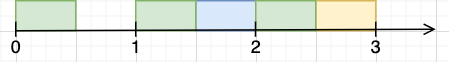
\includegraphics[width=3in]{images/timeline-flatten}
   \caption{Unfolded timeline}
   \label{timeline-flatten}
   \end{figure}

Analytically the system utilisation is approximately $\sum_{i \in \{RP, OCP, ALR\}}{C_i \over T_i} = {0.5 \over 1} + {0.5 \over 3} + {0.5 \over 3} = {5 \over 6}$. Runtime overhead, such as system ticker or context switch, and also blocking times have been left out the formula given that they are negligible in the approximation.

\section{EDF Analysis}

The EDF scheduling is a dynamic-priority algorithm that assigns priorities to individual jobs of a task based on its absolute deadline.
EDF, in contrast to FPS, is an optimal scheduler and can handle a total utilization less or equal to 1.

Before we go any further, there are two issues to be addressed.

First, as mentioned in chapter 7, MAST demands further restrictions for EDF analysis tools.
To keep consistency between Gee model and application, we had to discard Offset\_Based\_Approx and Holistic tools:
The former rollback to the latter, the latter lacks shared resources support.
The last standing option was EDF\_monoprocessor tool which implements the exact response time analysis for single-processor EDF systems.
We are restricted to Simple\_Transaction\_Only and to be compliant, only an independent task set can be modeled.
In addition, EDF\_monoprocessor doesn't allow to take into account jitter related to system ticker.
%We believe this is due to the inability to handle an interrupt without the notion of priority, stranger to EDF scheduling.

The synchronization protocol required by EDF\_monoprocessor is the well known Stack Resource Policy, while the runtime implementation uses the Deadline Floor Protocol (DFP).
DFP is an EDF counterpart of IPCP, as outlined in section 1.1.
Indeed, rather than assigning a ceiling priority to each shared resource, a deadline floor is computed and rather than raising the priority of a task to the resource's ceiling,
the task reduces its current deadline to reflect the floor value of the resource.
The deadline floor of a resource is computed as the minimum relative deadline of any task accessing such resource.
Nevertheless, the above disparity in resource access control can be ignored because of the worst-case behavior equivalence among SRP and DFP.
Indeed they lead to the same blocking time in the scheduling analysis.

To write down an EDF MAST model, the preemption level for each Task must be defined according to SRP.
A preemption level is inversely proportional to the Task relative deadline.

\begin{table}[!htbp]
   \centering
   \begin{tabular}{lllll}
     \toprule
     Task name & Deadline (ms) & Preemption Level \\
     \midrule
     External\_Event\_Server & 100 & 40 \\
     Regular\_Producer & 500 & 30 \\
     On\_Call\_Producer & 800 & 20 \\
     Activation\_Log\_Reader & 1000 & 10 \\
     \bottomrule
   \end{tabular}
   \caption{Task set suggested Preemption Levels}
   \label{tab:tasks-attributes}
\end{table}

The next step is to define a ceiling preemption level for each resource as the highest preemption level between any task accessing the resource.

\begin{table}[!htbp]
   \centering
   \begin{tabular}{lllll}
     \toprule
     Resource name & Ceiling Preemption Level \\
     \midrule
     Request\_Buffer & 30 \\
     Activation\_Log & 40 \\
     Event\_Queue    & ?  \\
     \bottomrule
   \end{tabular}
   \caption{Resource set Ceiling Preemption Levels}
   \label{tab:tasks-attributes}
\end{table}



\section{Conclusions}

Non funziona mai un cazzo.

\bibliographystyle{unsrt}
%\bibliography{references}  %%% Remove comment to use the external .bib file (using bibtex).
%%% and comment out the ``thebibliography'' section.


%%% Comment out this section when you \bibliography{references} is enabled.
\begin{thebibliography}{1}

\bibitem{ycs}
A Burns, B Dobbing, T Vardanega.
\newblock "Guide for the use of the Ada Ravenscar Profile in high integrity systems".
\newblock In {\em University of York Technical Report YCS-2003-348}. January 2003.

\bibitem{ork}
Juan A. de la Puente, José F. Ruiz, Juan Zamorano.
\newblock "Open Ravenscar Real-Time Kernel. Design Definition File, Software Design Document".
\newblock 2001.

\bibitem{mast}
M. Gonzalez Harbour, J.J. GutiCrrez Garcia, J.C. Palencia GutiCrrez, and J.M. Drake Moyano.
\newblock "MAST Modeling and Analysis Suite for Real Time Applications".
\newblock In {\em Proceedings 13th Euromicro Conference on Real-Time Systems}. 2001.

\bibitem{ada-pcp}
Albert M. K. Cheng, James Ras.
\newblock "The Implementation of the Priority Ceiling Protocol in Ada-2005".
\newblock In {\em ACM SIGAda Ada Letters}. Volume XXVII Issue 1, pp 24-39. 2007.

\bibitem{mast-description}
J. M. Drake, M. G. Harbour, J. J. Gutiérrez, P. L. Martínez, J. L. Medina, J. C. Palencia
\newblock "Description of the MAST Model".
\newblock \url{https://mast.unican.es/mast_description.pdf}

\bibitem{mast-analysis}
J. M. Drake, M. G. Harbour, J. J. Gutiérrez, P. L. Martínez, J. L. Medina, J. C. Palencia
\newblock "MAST Analysis Techniques".
\newblock \url{https://mast.unican.es/mast_analysis_techniques.pdf}

\bibitem{mast-restrictions}
J. M. Drake, M. G. Harbour, J. J. Gutiérrez, P. L. Martínez, J. L. Medina, J. C. Palencia
\newblock "MAST Restrictions".
\newblock \url{https://mast.unican.es/mast_restrictions.pdf}

\bibitem{overrundetection}
Juan Zamorano, Alejandro Alonso, José Antonio Pulido, Juan Antonio de la Puente.
\newblock "Implementing Execution-Time Clocks for the Ada Ravenscar Profile".
\newblock In {\em Reliable Software Technologies - Ada-Europe 2004}. pp 132-143. Ada-Europe 2004.

\bibitem{absolute-delay}
Juan Zamorano, Jose F. Ruiz, Juan Antonio de la Puente.
\newblock "Implementing Ada.Real Time.Clock and Absolute Delays in Real-Time Kernels".
\newblock In {\em Reliable SoftwareTechnologies — Ada-Europe 2001}. pp 317-327. Ada-Europe 2004.

\bibitem{rm-dm}
Jane W. S. W. Liu.
\newblock "Rate-Monotonic and Deadline-Monotonic Algorithms".
\newblock In {\em Real-Time Systems}. pp 118-119. 2001.

\bibitem{critical-instants}
Jane W. S. W. Liu.
\newblock "Critical Instants".
\newblock In {\em Real-Time Systems}. pp 131-134. 2001.

\bibitem{optimality-rm-dm}
Jane W. S. W. Liu.
\newblock "Optimality of the RM and DM algorithms".
\newblock In {\em Real-Time Systems}. pp 118-119. 2001.

\bibitem{pcp-blocking}
Jane W. S. W. Liu.
\newblock "Basic Priority Ceiling Protocol - Duration of Blocking".
\newblock In {\em Real-Time Systems}. pp 295-296. 2001.

\bibitem{limited-priorities}
Jane W. S. W. Liu.
\newblock "Limited-Priority Levels".
\newblock In {\em Real-Time Systems}. pp 166-168. 2001.

\bibitem{tick-scheduling}
Jane W. S. W. Liu.
\newblock "Tick Scheduling".
\newblock In {\em Real-Time Systems}. pp 168-171. 2001.

\bibitem{anomalies-multiprocessor}
Jane W. S. W. Liu.
\newblock "Anomalous Behavior of Priority-Driven Systems".
\newblock In {\em Real-Time Systems}. pp 72-73. 2001.

\bibitem{hierarchical-scheduling}
Jane W. S. W. Liu.
\newblock "Schedulability Test of Hierarchically Scheduled Periodic Tasks".
\newblock In {\em Real-Time Systems}. pp 177-179. 2001.

\bibitem{debug-trace}
Joseph Yiu.
\newblock "Introduction to the Debug and Trace Features".
\newblock In {\em The Definitive Guide to ARM CORTEX-M3 and CORTEX-M4 Processors}. Chapter 4 pp 443-485. 2014.

\bibitem{semihosting}
Joseph Yiu.
\newblock "Semi-hosting".
\newblock In {\em The Definitive Guide to ARM CORTEX-M3 and CORTEX-M4 Processors}. Chapter 18.3 pp 591-595. 2014.

\bibitem{pendsv}
Joseph Yiu.
\newblock "PendSV exception".
\newblock In {\em The Definitive Guide to ARM CORTEX-M3 and CORTEX-M4 Processors}. Chapter 18.3 pp 591-595. 2014.

\bibitem{holistic-analysis}
KenTindell, JohnClark.
\newblock "Holistic schedulability analysis for distributed hard real-time systems".
\newblock In {\em Microprocessing and Microprogramming}. Volume 40, Issues 2–3, pp 117-134. April 1994.

\bibitem{liu-utilisation-bound}
C. L. Liu, James W. Layland.
\newblock "Scheduling Algorithms for Multiprogramming in a Hard-Real-Time Environment".
\newblock In {\em Journal of the ACM}. Volume 20 Issue 1, pp 46-61. Jan. 1973.

\bibitem{practitioner}
Klein, M., Ralya, Th., Pollak, B., Obenza, R., Harbour, M.G. .
\newblock "A Practitioner's Handbook for Real-Time Analysis". 1993.

\bibitem{practitioner-utilisation-bound}
Klein, M., Ralya, Th., Pollak, B., Obenza, R., Harbour, M.G. .
\newblock "Using Utilization Bounds for Each Event when Deadlines Are Within the Period".
\newblock In {\em A Practitioner's Handbook for Real-Time Analysis
}. chapter 4.1.2. 1993.

\bibitem{practitioner-growth}
Klein, M., Ralya, Th., Pollak, B., Obenza, R., Harbour, M.G. .
\newblock "Calculating Growth by Increasing Resource Usage of All Events".
\newblock In {\em A Practitioner's Handbook for Real-Time Analysis
}. chapter 4.3.8. 1993.

\bibitem{practitioner-common-data}
Klein, M., Ralya, Th., Pollak, B., Obenza, R., Harbour, M.G. .
\newblock "Designing Tasks that Must Synchronize to Share Common Data".
\newblock In {\em A Practitioner's Handbook for Real-Time Analysis
}. chapter 5.2. 1993.

\bibitem{effects-runtime}
Klein, M., Ralya, Th., Pollak, B., Obenza, R., Harbour, M.G. .
\newblock "Effects of Operating System and Runtime Services on Timing Analysis".
\newblock In {\em A Practitioner's Handbook for Real-Time Analysis
}. chapter 7. 1993.

\bibitem{interrupt-handler}
Klein, M., Ralya, Th., Pollak, B., Obenza, R., Harbour, M.G. .
\newblock "Service the Event at a Specified Software Priority".
\newblock In {\em A Practitioner's Handbook for Real-Time Analysis
}. chapter 5.3.5.2. 1993.

\bibitem{ada-tasks}
Alan Burns, Andy Wellings.
\newblock "Scheduling real-time systems - Fixed Priority Dispatching".
\newblock In {\em Concurrent and real-time programming in Ada}. chapter 13.1. 2007.

\bibitem{timing-events}
Alan Burns, Andy Wellings.
\newblock "Timing events".
\newblock In {\em Concurrent and real-time programming in Ada}. chapter 15.2. 2007.

\bibitem{timing-properties}
Enrico Mezzetti, Marco Panunzio, Tullio Vardanega.
\newblock "Preservation of Timing Properties with the Ada Ravenscar Profile".
\newblock In {\em Reliable Software Technologiey – Ada-Europe 2010}. pp 153-166. 2010.

\bibitem{etc}
Kristoffer Nyborg Gregertsen, Amund Skavhaug.
\newblock "Implementation and Usage of the new Ada 2012 Execution Time Control Features".
\newblock In {\em Ada User Journal}. 2011.

\bibitem{pessimistic-rma}
J.C. Palencia ; M. Gonzalez Harbour.
\newblock "Schedulability analysis for tasks with static and dynamic offsets".
\newblock In {\em Proceedings 19th IEEE Real-Time Systems Symposium}. 1998.

\bibitem{tindell-offsets}
K. Tindell.
\newblock "Adding Time - Offsets to Schedulability Analysis".
\newblock Technical Report YCS 221, Dept. of Computer Science, University of York, England, January 1994.

\bibitem{wcet-problem}
R. Wilhelm et al..
\newblock "The worst-case execution-time problem—overview of methods and survey of tools".
\newblock In {\em Trans. on Embedded Computing Sys}. vol. 7, no. 3, pp. 153, 2008.

\bibitem{spuri}
M. Spuri.
\newblock "Analysis of Deadline Scheduled Real-Time Systems".
\newblock In {\em [Research Report] RR-2772, INRIA}. 1996.

\end{thebibliography}


\end{document}
